\documentclass[10pt]{beamer}

\usepackage{listing}
\usepackage{minted}

\usepackage{pgfpages}
\usepackage{verbatim}
\usepackage{amsmath}
\usepackage{amssymb}
\usepackage{setspace}
\usepackage{soul}
\usepackage[normalem]{ulem}

\usepackage{graphicx}
% \usepackage{amssymb}
% \usepackage{amsmath}
\usepackage{amsthm}
\usepackage{lscape}
\usepackage{verbatim}
\usepackage{enumerate}
\usepackage{afterpage}
\usepackage{tikz}
\usepackage{listings}
\usepackage{listing}
\usepackage{circuitikz}
\usepackage{todonotes}
\usepackage{url}
\usepackage{rotating}
\usepackage{subfigure}
\usepackage{algpseudocode}
\usepackage{algorithm}
\usepackage{wasysym}
\usepackage{amssymb}% http://ctan.org/pkg/amssymb
\usepackage{pifont}% http://ctan.org/pkg/pifont
\newcommand{\cmark}{\ding{51}}%
\newcommand{\xmark}{\ding{55}}%

\usetikzlibrary{dsp,chains}

\setcounter{MaxMatrixCols}{20}

% \usepackage{hyperref}
% \usepackage{minted}
% \usepackage{mdframed}
% \usepackage[all,defaultlines=3]{nowidow}

% \usetikzlibrary{dsp,chains}

% \newtheorem{definition}{Definition}
% \newtheorem{thm}{Theorem}


\setbeamercovered{dynamic}
% \mode<presentation>{\usepackage{beamer}}
%\pgfpagesuselayout{4 on 1}[a4paper,border shrink=5mm]

\newcommand{\field}[1]{\mathbb{#1}} %requires amsfonts

\usetheme{Antibes}
\usecolortheme{beaver}
\title[Large Substitution Boxes with Efficient Combinational Implementations]{Large Substitution Boxes with Efficient Combinational Implementations}

\usepackage{mathptmx}
\usepackage[scaled=.90]{helvet}
\usepackage{courier}
\usepackage[T1]{fontenc}

%\pgfpagesuselayout{4 on 1}[letterpaper,border shrink=5mm]

\institute[RIT]{}
\date{\today}
%\subtitle{}
\author[Christopher A. Wood]{Christopher A. Wood \\ Department of Computer Science \\ Rochester Institute of Technology \\ \vspace{1em} {\scriptsize Now: {\tt caw4567@rit.edu} \\ Soon: {\tt woodc1@uci.edu}} \\ \vspace{2em}
{\scriptsize Advisor: Stanis{\l}aw Radziszowski \\ Reader: Marcin Lukowiak \\ Observer: Alan Kaminsky \\ Observer: Michael Kurdziel}
}
%\institute[]{}
\date{August 9, 2013}

\begin{document}

\begin{frame}
	\titlepage
\end{frame}

\begin{frame}
	\frametitle{Agenda}
	\tableofcontents
\end{frame}


%%%%%%%%%%%%%%%%% OUTLINE
\section{Introduction, Motivation, Review}
\begin{frame}
	\frametitle{Security from an Information Theory Perspective}
	According to Shannon, cryptographic algorithms were secure if they yielded high measures of confusion and diffusion:
	\begin{itemize}
		\item \emph{Confusion} - complex relationship between the secret key and ciphertext
		\item \emph{Diffusion} - dissipation of plaintext bits throughout ciphertext bits
	\end{itemize}
\end{frame}

% Review of AES
% \subsection{Rijndael Review}
\begin{frame}
	\frametitle{Rijndael - The Advanced Encryption Standard}
	Let's take a look at the inner workings of Rijndael (AES) from Shannon's perspective
	\begin{itemize}
		\item Diffusion (linear operations):
		\begin{itemize}
			\item Shift rows
			\item Mix columns
			\item Add round key
		\end{itemize}
		\item Confusion (nonlinear operations):
		\begin{itemize}
			\item Substitute bytes
		\end{itemize}
	\end{itemize}
\end{frame}

% \begin{frame}
% 	\frametitle{The AES S-Box}
% 	The S-box is the \emph{only} source of nonlinearity in the AES, defined as follows:
% \begin{align*}
% S(x) =  
% \begin{pmatrix}
% 1 & 0 & 0 & 0 & 1 & 1 & 1 & 1 \\
% 1 & 1 & 0 & 0 & 0 & 1 & 1 & 1 \\
% 1 & 1 & 1 & 0 & 0 & 0 & 1 & 1 \\
% 1 & 1 & 1 & 1 & 0 & 0 & 0 & 1 \\
% 1 & 1 & 1 & 1 & 1 & 0 & 0 & 0 \\
% 0 & 1 & 1 & 1 & 1 & 1 & 0 & 0 \\
% 0 & 0 & 1 & 1 & 1 & 1 & 1 & 0 \\
% 0 & 0 & 0 & 1 & 1 & 1 & 1 & 1 \\
% \end{pmatrix}
% \begin{pmatrix}
% x_0 \\
% x_1 \\
% x_2 \\
% x_3 \\
% x_4 \\ 
% x_5 \\
% x_6 \\
% x_7 \\
% \end{pmatrix}^{-1}
% +
% \begin{pmatrix}
% 1 \\
% 1 \\
% 0 \\
% 0 \\
% 0 \\ 
% 1 \\
% 1 \\
% 0 \\
% \end{pmatrix}
% \end{align*}

% 	\medskip

% 	\begin{center}
% 	Inversion is in the Galois field $GF(2^8)$
% 	\end{center}

% \end{frame}

\begin{frame}
	\frametitle{The Importance of the S-Box}
	Why bother with the S-box?
	\begin{itemize}
		\item In Substitution-Permutation algorithms, the S-box is typically the only nonlinear operation
		\begin{itemize}
			\item Reasonably sized linear systems of equations are easy to solve
			\item Nonlinearity provides resistance to many known attacks
		\end{itemize}
		\pause
		\item S-boxes are used in both the DES and AES
		\pause
		\item They can be implemented ``efficiently'' in both hardware (as we will show) and software
		\begin{itemize}
			\item Secure implementations are not a part of this work. We assume precautions are taken to mitigate side-channel attacks.
		\end{itemize}
	\end{itemize}
\end{frame}

\begin{frame}
	\frametitle{Why Bother Going Bigger?}
	Why study at 16-bit S-boxes?
	\begin{itemize}
		\item They might be useful in the future
		\begin{itemize}
			\item Will the size of internal elements in the next block cipher standard bump up to 16-bits?
		\end{itemize}
		\pause
		\item To determine if such implementations are feasible or practical
		\begin{itemize}
			\item LUTs for 16-bit S-boxes are out of the question.
		\end{itemize}
		\pause
		\item It may offer insight into new perspectives of S-box constructions and implementation techniques
	\end{itemize}
\end{frame}

%%%% SECURITY NEED
\begin{frame}
	\frametitle{Constructing Cryptographically Strong S-boxes}
	\begin{itemize}
		\item Question 1: What constitutes a cryptographically strong S-box?
		\pause
		\medskip
		\begin{itemize}
			\item One that is not susceptible to known attacks
		\end{itemize}
		\pause
		\medskip
		% \item Question 2: How do we measure S-boxes to determine their resiliency to known attacks?
		\item Question 2: How do we build cryptographically strong S-boxes?
		\pause
		\medskip
		\begin{itemize}
			\item Choose constructions that have \emph{known} and \emph{measurable} security properties
		\end{itemize}
		\pause
		\medskip
		\item Question 3: How can we implement these S-boxes efficiently in hardware?
		\pause
		\medskip
		\begin{enumerate}
			\item Decompose the S-box calculation into bitwise operations
			\item Minimize the logic involved in these operations
		\end{enumerate}
	\end{itemize}
\end{frame}

% ARK: the actual encryption stage, XOR state matrix with appropriate key block in key schedule
% Implications: How much can we guarantee about the construction of the key schedule? Implies there are good and bad keys that can be used. The algorithm should not have to worry about the usage of a "good" key to be secure.
% \begin{frame}
% 	\frametitle{Add Round Key}
% 	\begin{center}
%       		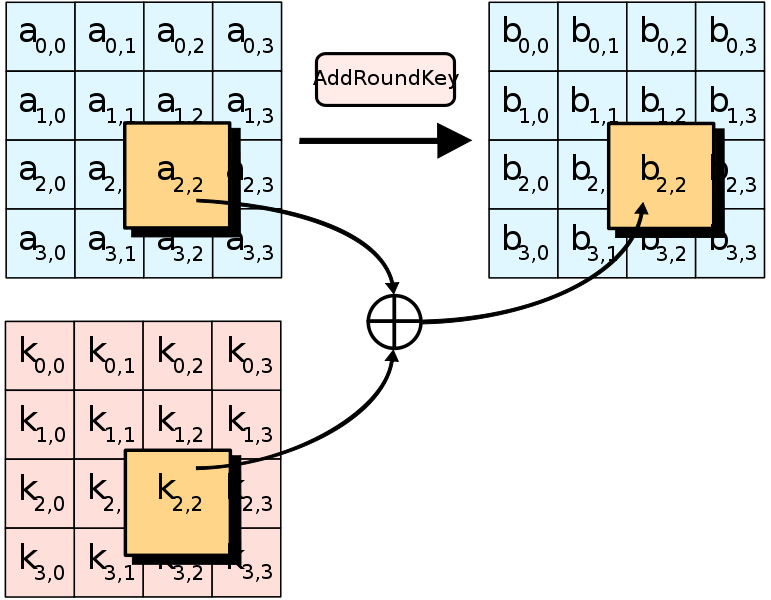
\includegraphics[width=75mm]{images/ark.png}
% 	\end{center}
% \end{frame}

% % purpose: just another permutation for diffusion... just rotate the data to avoid linear cryptanalysis. nothing special
% \begin{frame}
% 	\frametitle{Shift Rows}
% 	\begin{center}
%       		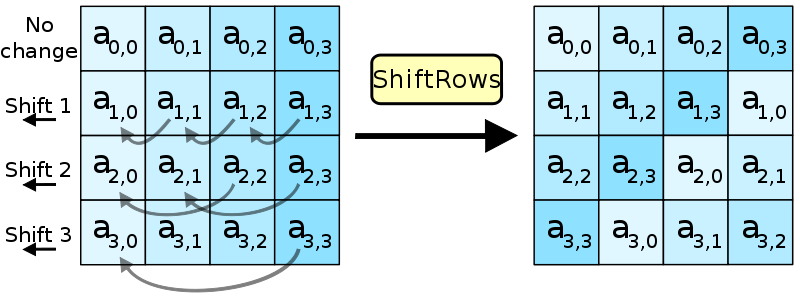
\includegraphics[width=75mm]{images/shift.png}
% 	\end{center}
% \end{frame}

% \begin{frame}
% 	\frametitle{Mix Columns}
% 	\begin{center}
%       		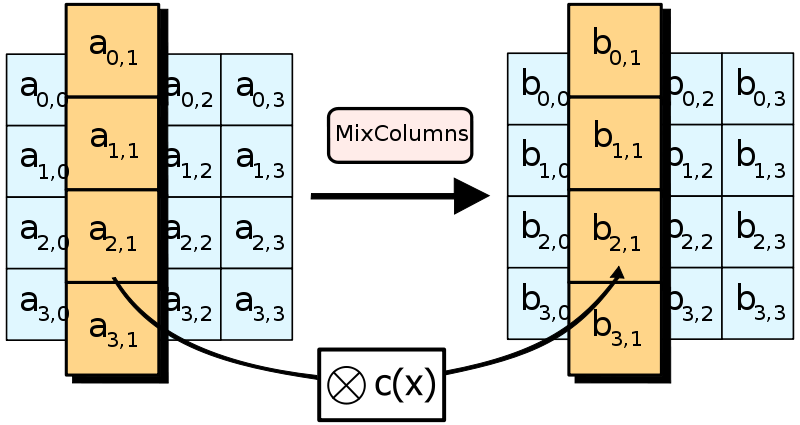
\includegraphics[width=75mm]{images/mix.png}
% 	\end{center}
% \end{frame}

% \begin{frame}
% 	\frametitle{Substitute Bytes} %guarantees about branch number (# of active s-boxes) and the measure of nonlinearity 
% 	\begin{center}
%       		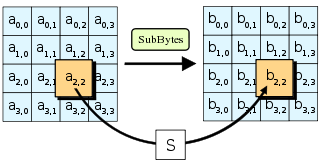
\includegraphics[width=75mm]{images/sub.png}
% 	\end{center}
% \end{frame}

% \begin{frame}
% 	\frametitle{Substitute Bytes}
% 	This affine transformation can also be represented algebraically as follows
% 	\begin{eqnarray*}
% 		b_i' = b_i \oplus b_{(i+4) mod 8} \oplus b_{(i+5) mod 8} \oplus b_{(i+6) mod 8} \oplus b_{(i+7) mod 8} \oplus c_i
% 	\end{eqnarray*}
% 	where $i$ is the $i$th bit of the input byte $b$ and $c = \langle 01100011 \rangle$.
% \end{frame}

% \begin{frame}
% 	\frametitle{Substitution Permutation Networks}
% \end{frame}

%%%%% TODO: DEFINITIONS HERE
% galois fields, composite fields, bases, boolean functions, etc
%%%%%

\begin{frame}
	\frametitle{Galois Fields}
	\begin{itemize}
		\item A Galois field $GF(\cdot)$ is just a finite field of $p$ ($GF(p)$) or $p^n$ ($GF(p^n)$) elements, where $p$ is prime
		\item The field's characteristic is the smallest non-negative integer $k$ such that $\underbrace{a + a + \dotsb + a}_{k \text{ times}} = 0$
		\item We focus on Galois fields with characteristic $2$ - $GF(2^n)$ - as elements are easily represented as bit strings in hardware and software
		\item We say that $GF(2^n)$ is an $n$ degree extension of $GF(2)$ (the subfield)
	\end{itemize}
\end{frame}

\begin{frame}
	\frametitle{Composite Galois Fields}
	Composite fields are simply fields composed of \emph{more than one extension}!

	\medskip

	Let $k = n \times m$

	\medskip

	$GF((2^n)^m)$ (mod $p(v), q(w)$) is a composite field isomorphic to $GF(2^k)$ (mod $r(x)$) if the following are true:
	\begin{itemize}
		\item $GF(2^n)$ is an $n$ degree extension of $GF(2)$ by an $n$ degree irreducible polynomial $p(v)$ over $GF(2)$
		\item $GF((2^n)^m)$ is an $m$ degree extension of $GF(2^n)$ by an $m$ degree irreducible polynomial $q(w)$ over $GF(2^n)$
		\item $GF(2^k)$ is a $k$ degree extension of $GF(2)$ by an $k$ degree irreducible polynomial $r(x)$ over $GF(2)$
	\end{itemize}
\end{frame}

\begin{frame}
	\frametitle{Bases of Galois Fields}
It is natural to represent an element $\alpha \in GF(p^n)$ as a polynomial of the form
\begin{align*}
\alpha = a_{n-1}x^{n-1} + a_{n-2}x^{n-2} + ... + a_2x^2 + a_1x + a_0,
\end{align*}
where $a_i \in GF(p)$ are the coefficients of the polynomial. 
\pause
\begin{center}
This is the polynomial basis representation.
\end{center}
\end{frame}

\begin{frame}
	\frametitle{Bases of Galois Fields (continued)}
	Let $\theta$ be a root of $p(x)$, the irreducible polynomial defining $GF(p^n)$, and let $\alpha \in GF(p^n)$
	\pause
	\begin{itemize}
		\item Polynomial basis: $[\theta^0,\theta^i,\dots,\theta^{n-1}]$
		\begin{align*}
			\alpha = a_{n-1}\theta^{n-1} + a_{n-2}\theta^{n-2} + \dotsb + a_{1}\theta + a_0
		\end{align*}
		\pause
		\item Normal basis: $[\theta^{p^{0}},\theta^{p^{1}},\dots,\theta^{p^{n-1}}]$
		\begin{align*}
			\alpha = a_{n-1}\theta^{p^{n-1}} + a_{n-2}\theta^{p^{n-2}} + \dotsb + a_{p^{1}}\theta^{p} + a_0\theta
		\end{align*}
	\end{itemize}

	\medskip 
	\begin{center}
		(Note: $a_i \in GF(p)$)
	\end{center}
\end{frame}

\begin{frame}
	\frametitle{Boolean Functions}
	A Boolean function $f$ is simply a function of the form:
	\begin{align*}
		f : \mathbb{F}_2^n \to \mathbb{F}_2
	\end{align*}

	\medskip
	\pause

	We may represent a Boolean function in the following ways:
	\begin{itemize}
		\item Truth table: 
		\begin{align*}
			f(x_0,\dots,x_n) = (f(\bar{0}), \dots, f(\bar{1}))
		\end{align*}
		\item Algebraic Normal Form (ANF): 
		\begin{align*}
			f(x_0,\dots,x_{n-1}) = \bigoplus_{(a_0,\dots,a_{n-1}) \in \mathbb{F}_2^n} h(a_0,\dots,a_{n-1})x_0^{a_0}x_1^{a_1}\dots x_{n-1}^{a_{n-1}}
		\end{align*}
	\end{itemize}

	\medskip
	\pause
	S-boxes from $\mathbb{F}_2^n \to \mathbb{F}_2^m$ may be viewed as $(n,m)$ Boolean functions
\end{frame}

% \begin{frame}
% 	\frametitle{Walsh Transform}
% 	The Walsh transform $W_f(x)$ is a very useful function to be used with Boolean functions

% 	\begin{align*}
% 		W_f(\bar{w}) & = \sum_{\bar{x} \in \mathbb{F}_2^n}(-1)^{f(\bar{x}) \oplus \bar{x}\cdot\bar{w}} \\
% 		& = 2^n - 2 \times \text{HW}(f(\bar{x}) \oplus \bar{x} \cdot \bar{w}).
% 	\end{align*}

% 	The Walsh transform effectively generates few higher magnitude coefficients from a more compact signal (i.e. the truth table)
% \end{frame}

% Attacks
\section{Security Properties of the S-Box}
\begin{frame}
	\frametitle{Common Attacks}
	\begin{itemize}
		\item Linear cryptanalysis
		\item Differential cryptanalysis
		\item Algebraic attacks
		\item Interpolation attacks
		\item ... and more
	\end{itemize}
\end{frame}

%% nonlinearity
\begin{frame}
	\frametitle{Linear Cryptanalysis}
	Linear cryptanalysis exploits a high (or low) probability that some linear combination of input and output bits in the S-box is satisfied

	\medskip
	\pause

	What makes an S-box susceptible to this type of attack?

	\pause 
	\medskip

	\begin{center}
		\emph{Low nonlinearity}
	\end{center}


\end{frame}
% \begin{frame}
% 	\frametitle{Linear Cryptanalysis - Resistance}
% 	\begin{center}
% 		What makes an S-box susceptible to this type of attack?
% 	\end{center}

% 	\pause 

% 	\medskip

% 	\begin{center}
% 		\emph{Low nonlinearity}
% 	\end{center}
% \end{frame}
\begin{frame}
	\frametitle{S-Box Nonlinearity}
	The \emph{nonlinearity} of an $(n, m)$ S-box $S$, denoted as $\mathcal{N}_l(S)$, is defined as follows:

	\begin{align*}
		\mathcal{N}_l(S) & = \min_{c \in \mathbb{F}_2^m}\{\mathcal{N}_l(c \cdot S)\} = \min_{c \in \mathbb{F}_2^m}\{\mathcal{N}_l(c_0f_0 \oplus c_1f_1 \oplus \dotsb \oplus c_{m-1}f_{m-1})\},
	\end{align*}
	
	\medskip

	where $f_0,\dots,f_{m-1}$ are the $m$ coordinate functions of $S$ and 
	\begin{align*}
		N_l(f) & = \min_{\phi \in \Omega_n} d(f, \phi)\\
		& = 2^{n-1} - \frac{1}{2}\max_{u \in \mathbb{F}_2^n}|W_f(u)|
	\end{align*}
\end{frame}

% \begin{frame}
% 	\frametitle{The Fast Walsh Transform}
% 	\begin{itemize}
% 		\item We can quickly and efficiently compute the \emph{Walsh Spectrum} of a Boolean function $f$ using the Fast Walsh Transform
% 	\end{itemize}

% 	%% TODO: include the tikz image here
% \end{frame}

% differential uniformity
\begin{frame}
	\frametitle{Differential Cryptanalysis}
	\begin{itemize}
		\item Differential cryptanalysis exploits output differences that occur with high probability for each round of a cipher

		\pause 
		\item Put another way: Frequently occurring differences mean there exists a value $\beta \in GF(2^k)$ such that for any two randomly selected input elements $x$ and $\alpha$, $S(x + \alpha) + S(x) = \beta$

		\pause
		\item An ideal block cipher will have perfectly uniform differentials
	\end{itemize}

	\pause
	\medskip
	What makes an S-box susceptible to this type of attack?

	\pause 
	\medskip

	\begin{center}
		\emph{``High'' differential uniformity}
	\end{center}
\end{frame}

\begin{frame}
	\frametitle{Differential Uniformity}
	An S-box $S : GF(2^n) \to GF(2^m)$ is $\delta$-differentially uniform if for all $\alpha \in GF(2^n)$ and $\beta \in GF(2^m)$ we have
	\begin{align*}
		|\{x \in GF(2^n) | S(x + \alpha) + S(x) = \beta\}| \leq \delta, 
	\end{align*}

	\medskip
	\pause
	\begin{itemize}
		\item There exists many known $(n, m)$ S-boxes with low values of $\delta$ (i.e. 1 - perfectly nonlinear - or 2 - almost perfectly nonlinear)
		\pause
		\item They are \emph{rarely} used! The inverse power mapping has $\delta = 4$, which is low enough for cryptographic purposes
	\end{itemize}
\end{frame}

\begin{frame}
	\frametitle{Other Well Known Attacks}
	\begin{itemize}
		\item Algebraic attacks
		\begin{itemize}
			\item Goal: define the cipher as (large) system of \emph{linearized} equations with key-dependent coefficients to solve 
			\item Relevant metric: algebraic immunity
			\begin{itemize}
				\item Dependent on the number of affine equations and monomials present in the linearized system
				\item Both can be calculated in $\mathcal{O}(n^2)$ time
			\end{itemize}
		\end{itemize}
		\pause
		\item Interpolation attacks
		\begin{itemize}
			\item Goal: model the cipher as a high-order polynomial with key-dependent coefficients and solve
			\item Relevant metric: algebraic complexity
			\begin{itemize}
				\item Proportional to the number of terms in the unique interpolation polynomial representing the S-box
				\item Can be determined using Lagrangian interpolation
			\end{itemize}
		\end{itemize}
	\end{itemize}
\end{frame}

%% Algebraic attacks XL and XSL
% \begin{frame}
% 	\frametitle{Algebraic Attacks}
% 	\begin{itemize}
% 		\item These attacks try to represent the block cipher (S-box included) as a system of multivariate equations over $GF(2)$ and solve.
% 		\item Systems obtained through linearization techniques are often too complex to solve
% 		\item The attack is \emph{not} dependent on the number of rounds used in a cipher
% 	\end{itemize}

% 	\pause
% 	\medskip
% 	What makes an S-box susceptible to this type of attack?

% 	\pause 
% 	\medskip

% 	\begin{center}
% 		\emph{High numbers of affine equations present in the linearized system and a small number monomials in the system}
% 		% This is a result of the number of algebraic representation of the S-box, and is entirely \emph{independent} from the number of rounds in the cipher!
% 	\end{center}
% \end{frame}

% \begin{frame}
% 	\frametitle{Algebraic Immunity}
% 	With the ``new'' XSL linearization attack on block ciphers that exploit their sparse structure, algebraic immunity has evolved to be defined as follows:
% 	\begin{align*}
% 		\Gamma(r, s, t) & = (t/s)^{\lceil t/r \rceil} \\
% 		\Gamma'(r,s,t) &= ((t - r)/s)^{\lceil (t - r)/s \rceil},
% 	\end{align*}
% 	where 
% 	\begin{itemize}
% 		\item $r$ is the number of equations in the linearized S-box representation,
% 		\item $s$ is the dimension of the S-box (i.e. $GF(2^s)$), and
% 		\item $t$ is the number of terms in the spare representations
% 	\end{itemize}
% \end{frame}

% %% Interpolation attacks
% \begin{frame}
% 	\frametitle{(Less Common) Interpolation Attacks}
% 	\begin{itemize}
% 		\item Similar in spirit to algebraic attacks
% 		\item Try to model the entire cipher as a higher-order polynomial with key-dependent coefficients
% 		\item Solving for these coefficients can reveal information about the key
% 	\end{itemize}
% \pause
% We solve this system with Lagrangian interpolation
% \begin{align*}
% p(x) = \sum_{i=1}^{n} y_i \prod_{1 \leq j \leq n, j \not= i} \frac{x - x_j}{x_i - x_j}.
% \end{align*}

% \pause
% 	\medskip
% 	What makes an S-box susceptible to this type of attack?

% 	\pause 
% 	\medskip

% 	\begin{center}
% 		\emph{Small number of terms in the interpolation polynomial}
% 	\end{center}
% \end{frame}

% \begin{frame}
% 	\frametitle{Algebraic Complexity}
% 	\begin{itemize}
% 	\item The larger the number of terms in the polynomial, the more difficult the attack becomes. 
% 	\item The AES is safe against this attack, which has the following polynomial:
% 	\scriptsize
% 	\begin{align*}
% 		p(x) = 05x^{254} + 09x^{253} + F9x^{251} + 25x^{247} + F4x^{239} + 01x^{223} + B5x^{191} + 8Fx^{127} + 63
% 	\end{align*}
% 	\normalsize
% 	\end{itemize}

% 	\medskip

% 	Morale: pick affine transformations for the S-box that increase the number of terms (algebraic complexity) in this interpolation polynomial
% \end{frame}

%% Other metrics
\begin{frame}
	\frametitle{Other Relevant Security Metrics}
	There are other important metrics by which we can assess the strength of cryptographic S-boxes:
	\begin{itemize}
		\item $t$-Resiliency
		\begin{itemize}
			\item Balanced outputs (i.e. bijective) and $t$-CI (correlation immunity)
			\item The output bit distribution remains unchanged when at most $t$ input bits are fixed
		\end{itemize}
		\item Branch number
		\begin{itemize}
			\item Estimating the cipher's measure of diffusion
		\end{itemize}
		\item Strict Avalanche Criteria (SAC) 
		\begin{itemize}
			\item Ensuring that $1/2$ of output bits change for every single input bit change
		\end{itemize}
	\end{itemize}
\end{frame}

%%%%% 
\begin{frame}
\frametitle{S-Box Constructions}
	\begin{itemize}
		\item \sout{Question 1: What constitutes a cryptographically strong S-box?}
		\medskip
		\begin{itemize}
			\item \sout{One that is not susceptible to known attacks}
		\end{itemize}
		\medskip
		% \item Question 2: How do we measure S-boxes to determine their resiliency to known attacks?
		\item Question 2: How do we build cryptographically strong S-boxes?
		\medskip
		\begin{itemize}
			\item Choose constructions that have \emph{known} and \emph{measurable} security properties
		\end{itemize}
	\end{itemize}
\end{frame}

\section{S-Box Constructions}
\begin{frame}
	\frametitle{Possible S-Box Constructions}
	We enforce the constraint that S-boxes are bijective functions from $\mathbb{F}_{2^n} \to \mathbb{F}_{2^n}$ (i.e. $(n,n)$ Boolean functions).

	\medskip

	Two very popular constructions are:
	\begin{itemize}
		\item Boolean functions
		\begin{itemize}
			\item Pros: Superb cryptographic properties (nonlinearity, differential uniformity, correlation immunity, resiliency, etc)
			\item Cons: Efficient implementations are difficult to obtain
		\end{itemize}
		\pause
		\item \textbf{Galois field power mappings}
		\begin{itemize}
			\item Combined with affine transformations for increased algebraic complexity
			\item Pros: simple algebraic expressions, well studied, \emph{basis of the AES S-box}
			\item Cons: Difficult to obtain ideal cryptographic properties that Boolean function constructions yield, but they are still good enough
		\end{itemize}
	\end{itemize}
\end{frame}

\begin{frame}
	\frametitle{Cryptographically Significant Power Mappings}
	Important properties of power mappings over $GF(2^n)$:
	\begin{itemize}
		\item Must be of the form $f(x) = x^d$
		\begin{itemize}
			\item They are usually characterized by their exponent $d$
		\end{itemize}
		\item Only bijective if $\gcd\{d, 2^n - 1\} = 1$
	\end{itemize}
\end{frame}

\begin{frame}
	\frametitle{Cryptographically Significant Power Mappings (continued)}
	There are many known cryptographically significant power mappings with ideal nonlinearity and differential uniformity:
	\begin{itemize}
		\item Gold: $2^{k} + 1$, $\gcd\{k,n\} = 1$ for some $1 \leq k \leq 2^{n} - 1$
		\item Kasami: $2^{2k} - 2^k + 1$, $\gcd\{k,n\} = 1$ for some $1 \leq k \leq n/2$
		\item Dobbertin: $2^{4k + 3k + 2k + k} - 1$ over $GF(2^n)$ with $n = 5k$
		\item Niho: $2^{m} + 2^{m/2} - 1$ over $GF(2^n)$ with $n = 2m + 1$ and $m$ even, $2^{m} + 2^{(3m + 1)/2} - 1$ over $GF(2^n)$ with $n = 2m + 1$ and $m$ odd
		\item Welch: $2^m + 3$ over $GF(2^n)$ with $n = 2m + 1$
		\item Inverse: $-1 \equiv 2^n - 2$
	\end{itemize}
\end{frame}

% Gold & $2^{k} + 1$, $\gcd\{k,n\} = 1$ for some $1 \leq k \leq 2^{n} - 1$ & \cite{Courtois05-1} \\ \hline
%     Kasami & $2^{2k} - 2^k + 1$, $\gcd\{k,n\} = 1$ for some $1 \leq k \leq n/2$ & \cite{Courtois05-1} \\ \hline
%     Dobertin & $2^{4k + 3k + 2k + k} - 1$ over $GF(2^n)$ with $n = 5k$ & \cite{Courtois05-1} \\ \hline
%     Niho & $2^{m} + 2^{m/2} - 1$ over $GF(2^n)$ with $n = 2m + 1$ and $m$ even & \cite{Courtois05-1} \\ 
%     ~ & $2^{m} + 2^{(3m + 1)/2} - 1$ over $GF(2^n)$ with $n = 2m + 1$ and $m$ odd & ~ \\ \hline
%     Welch & $2^m + 3$ over $GF(2^n)$ with $n = 2m + 1$ & \cite{Courtois05-1} \\ \hline

\begin{frame}
	\frametitle{Choosing the Right Mapping}
	What if $n = 16$?
	\begin{itemize}
		\item \sout{Gold: $2^{k} + 1$, $\gcd\{k,n\} = 1$ for some $1 \leq k \leq 2^{n} - 1$}
		\pause
		\item \sout{Kasami: $2^{2k} - 2^k + 1$, $\gcd\{k,n\} = 1$ for some $1 \leq k \leq n/2$}
		\pause
		\item \sout{Dobbertin: $2^{4k + 3k + 2k + k} - 1$ over $GF(2^n)$ with $n = 5k$}
		\pause
		\item \sout{Niho: $2^{m} + 2^{m/2} - 1$ over $GF(2^n)$ with $n = 2m + 1$ and $m$ even, $2^{m} + 2^{(3m + 1)/2} - 1$ over $GF(2^n)$ with $n = 2m + 1$ and $m$ odd}
		\pause
		\item \sout{Welch: $2^m + 3$ over $GF(2^n)$ with $n = 2m + 1$}
	\end{itemize}
	\pause
	\begin{center}
		\emph{The inverse mapping is the only remaining candidate!}
	\end{center}
\end{frame}

\begin{frame}
	\frametitle{Affine Transformation Criteria}
	\begin{itemize}
		\item Affine transformations are used to increase the complexity of the algebraic representation of the S-box.
		\begin{itemize}
			\item Without an affine transformation, the algebraic representation would simply be $S(x) = x^d$
		\end{itemize}
		\pause
		\item AES-like S-boxes $S(x)$ have the form
		\begin{align*}
			S(x) & = A(P(x)) \\
			S^{-1}(x) & = P^{-1}(A^{-1}(x))
		\end{align*}
		where $P(x)$ is the inverse power mapping and $A(x)$ is the affine transformation
		\pause
		\item The maximum algebraic complexity (number of terms in the interpolation polynomial) of AES-like S-boxes over $GF(2^n)$ is $n + 1$
		\begin{itemize}
			\item This has proven sufficient for preventing interpolation attacks
		\end{itemize}
		\pause
		\item The final S-box should have no fixed points:
		\begin{align*}
			S(x) \oplus x = \{0\}^n \\
			S(x) \oplus x = \{1\}^n
		\end{align*}
	\end{itemize}
\end{frame}

\begin{frame}[fragile]
	\frametitle{Searching for Affine Transformations}
	Non-deterministic procedure for finding suitable affine transformations \\

	\medskip 

	\textbf{Input:} $GF(2^n), d, k$ \\
	\begin{enumerate}
		\item Generate a random matrix $\mathbf{A}$ over $GF(2)$
		\item If $det(\mathbf{A}) \not= 0$ go to step 1.
		\item Generate a random element $c \in GF(2^n)$ with weight $k$
		\item Iterate over every element $e \in GF(2^n)$ and compute $y = \mathbf{A}(e^d) + c$ and $y^{-1} = (\mathbf{A}^{-1}(y + c))^{d^{-1}}$. If $e$ yields a fixed point with $\mathbf{A}$ and $c$, go to step 1. Store $y$ and $y^{-1}$ in maps $S$ and $S^{-1}$.
		\item Perform Lagrangian interpolation to obtain $p(y)$ and $p^{-1}(y)$ for $S$ and $S^{-1}$.
		\item If $\#p(y) > n$ and $\#p^{-1}(y) > n$, return $\mathbf{A}$ and $c$, else go to step 1.
	\end{enumerate}
\end{frame}
% {\fontsize{10}{10}\selectfont
% % \begin{algorithm}[H]
% % \caption{AffineSearch($\mathbb{F}, n$)} \label{alg:affineSearch}
% \begin{algorithmic}[1]
% \State $done \gets False$
% \Repeat 
%   \State $\mathbf{A} \gets RandomMatrix(GF(2), n, n)$
%   \State $c \gets RandomElement(\mathbb{F})$
%   \If {$det(\mathbf{A}) \not= 0$} \Comment{Only consider invertible matrices}
%     \State $valid \gets True$
%     \For {\textbf{each} $e \in \mathbb{F}$}
%       \If {$e$ is not a fixed point}
%         \State Compute and store $S(e) = \mathbf{A}e + c$ and $S^{-1}(e) = \mathbf{A}^(-1)(e + c)$
%       \Else
%         \State $valid \gets False$
%         \State Break
%       \EndIf
%     \EndFor
%     \If {$valid = True$}
%       \State $p(y) \gets Interpolate(S(x))$
%       \State $p^{-1}(y) \gets Interpolate(S^{-1}(x))$
%       \If {$\#p(y) > n$ and $\#p^{-1}(y) > n$}
%         \State \Return $\mathbf{A}, c$
%       \EndIf
%     \EndIf
%   \EndIf
% \Until {$done = False$}
% \end{algorithmic}
% % \end{algorithm}
% }

\begin{frame}
\frametitle{Efficient S-Box Computations}
	\begin{itemize}
		\item \sout{Question 1: What constitutes a cryptographically strong S-box?}
		\medskip
		\begin{itemize}
			\item \sout{One that is not susceptible to known attacks}
		\end{itemize}
		\medskip
		% \item Question 2: How do we measure S-boxes to determine their resiliency to known attacks?
		\item \sout{Question 2: How do we build cryptographically strong S-boxes?}
		\medskip
		\begin{itemize}
			\item \sout{Choose constructions that have \emph{known} and \emph{measurable} security properties}
		\end{itemize}
		\medskip
		\item Question 3: How can we implement these S-boxes efficiently in hardware?
		\medskip
		\begin{enumerate}
			\item Decompose the S-box calculation into bitwise operations
			\item Minimize the logic involved in these operations
		\end{enumerate}
	\end{itemize}
\end{frame}

%%%% REDUCTION TO SUBFIELD INVERSION
\section{Computing the Multiplicative Inverse in a Galois Field}
\begin{frame}
	\frametitle{Computing the Multiplicative Inverse}
	\begin{itemize}
		\item Extended Euclidean algorithm
		\pause
		\item Fermat's Little Theorem: $x^{-1} \equiv x^{2^n - 2}$ in $GF(2^n)$
		\pause
		\item \textbf{Reduction to subfield inversion using composite fields}
		\pause
		\begin{itemize}
			\item Decomposition to arithmetic over $GF(2)$ 
			\pause
			\item Itoh-Tsujii inversion algorithm
		\end{itemize}
	\end{itemize}
\end{frame}

% \subsection{Direct Calculation over $GF(2)$ with Composite Fields}
\begin{frame}
	\frametitle{Isomorphic Composite Fields}
	% Consider the fields isomorphic to $GF(2^{16})$

\begin{figure}
\centering
\begin{tikzpicture}
[bend angle =60,inner sep=0pt, minimum size =10mm,very thick,
from/.style={<-},
towards/.style={->},
field/.style={},
thick,scale=0.6, every node/.style={transform shape}]
\node[field] (gf216) at (0,0) {$GF(2^{16})$};
\node[field] (gf282) at (-6,-2) {$GF((2^8)^2)$};
\node[field] (gf228) at (0,-2) {$GF((2^2)^8)$};
\node[field] (gf244) at (6,-2) {$GF((2^4)^4)$};
\node[field] (gf2422) at (-8,-4) {$GF(((2^4)^2)^2)$};
\node[field] (gf2422) at (-4,-4) {$GF(((2^2)^4)^2)$};
\node[field] (gf2224) at (4,-4) {$GF(((2^2)^2)^4)$};
\node[field] (gf22222) at (-6,-6) {$\mathbf{GF((((2^2)^2)^2)^2)}$};

\draw [->] (-1,-.25) -- (-5.75,-1.55);
\draw [->] (0,-.35) -- (0,-1.55);
\draw [->] (1,-.25) -- (5.75,-1.55);
\draw [->] (-6.75,-2.25) -- (-8,-3.75);
\draw [->] (-5.25,-2.25) -- (-4,-3.75);
\draw [->] (5.25,-2.25) -- (4,-3.75);
\draw [->] (-8,-4.5) -- (-6,-5.75);
\end{tikzpicture}
\end{figure}
\pause
\begin{center}
	We focus on $GF((((2^2)^2)^2)^2)$.
\end{center}
\end{frame}

\begin{frame}
	\frametitle{Galois Field Arithmetic Decompositions}
	With composite fields, coefficient arithmetic is performed over the subfield.

	\medskip
	\pause

	How do we go about determining the complexity of all relevant arithmetic operations?

	\medskip
	\pause

	Define arithmetic in the first extension of $GF(2)$ - $GF(2^2)$ - and then walk up the tower to $GF((((2^2)^2)^2)^2)$, constructed as follows:
	\begin{itemize}
		\item $GF(2^2) / p(v) = v^2 + v + 1$
		\item $GF((2^2)^2) / q(w) = w^2 + w + \Sigma$
		\item $GF(((2^2)^2)^2) / r(x) = x^2 + x + \Pi$
		\item $GF((((2^2)^2)^2)^2) / s(y) = y^2 + y + \Lambda$
	\end{itemize}
\end{frame}

\begin{frame}
	\frametitle{Inversion in $GF(2^2)$}
	Inversion in $GF(2)$ is trivial, so we start with the first extension:
	\begin{align*}
		GF(2^2) / p(v) = v^2 + v + 1
	\end{align*}

	\medskip
	For $\delta \in GF(2^2)$ and $\gamma \in GF(2)$. We may compute $\delta^{-1}$ as follows:
	\pause
	\begin{itemize}
		\item Polynomial basis $[1, V]$
		\begin{align*}
			\delta & = \gamma_1 v + \gamma_2 \\
			\delta^{-1} & = \gamma_1 v + (\gamma_1 + \gamma_2)
		\end{align*}
		\pause
		\item Normal basis $[V, V^2]$ (by Fermat's Little Theorem)
		\begin{align*}
			\delta & = \gamma_1 v^2 + \gamma_2 v \\
			\delta^{-1} & = \gamma_2 v^2 + \gamma_1 v
		\end{align*}
	\end{itemize}

	\pause
	Overall: Polynomial basis requires one XOR and normal basis is ``free'' (bit swap)

\end{frame}

\begin{frame}
	\frametitle{Inversion With More Extensions}
	Things become more complicated when $GF(2^2)$ is extended to larger fields. Let $\epsilon \in GF((2^2)^2)/q(w) = w^2 + w + \Sigma$, $\delta \in GF(2^2)$.
	\pause
	\medskip
	\begin{itemize}
		\item Polynomial basis $[1, W]$
		\begin{align*}
			\epsilon^{-1} = \delta_1(\delta_2^2 + \delta_1\delta_2 + \delta_1^2\Sigma)^{-1}w + (\delta_1 + \delta_2)(\delta_2^2 + \delta_1\delta_2 + \delta_1^2\Sigma)^{-1}
		\end{align*}
		\pause
		\item Normal basis $[W, W^4]$
		\begin{align*}
			\epsilon^{-1} = ((\delta_1\delta_2 + (\delta_1 + \delta_2)^2\Sigma)^{-1}\delta_2) w^4 + ((\delta_1\delta_2 + (\delta_1 + \delta_2)^2\Sigma)^{-1}\delta_1) w
		\end{align*}
	\end{itemize}

	% $\epsilon^{-1} = \delta_1(\delta_2^2 + \delta_1\delta_2 + \delta_1^2\Sigma)^{-1}w + (\delta_1 + \delta_2)(\delta_2^2 + \delta_1\delta_2 + \delta_1^2\Sigma)^{-1}$
\end{frame}

\begin{frame}[fragile]
	\frametitle{Corresponding Inversion Circuits - Polynomial Basis}

		\begin{align*}
			\epsilon^{-1} = \delta_1(\delta_2^2 + \delta_1\delta_2 + \delta_1^2\Sigma)^{-1}w + (\delta_1 + \delta_2)(\delta_2^2 + \delta_1\delta_2 + \delta_1^2\Sigma)^{-1}
		\end{align*}

% \begin{columns}[t]

% \begin{column}[t]{0.45\linewidth}
\begin{figure}[H]
\centering
\begin{tikzpicture}
	\matrix (m1) [row sep=2.5mm, column sep=5mm]
	{
		%--------------------------------------------------------------------
		\node[coordinate]                  (m00) {};          &
		\node[coordinate]                  (m01) {};          &
		\node[coordinate]                  (m02) {};          &
		\node[coordinate]                  (m03) {};          &
		\node[coordinate]                  (m04) {};          &
		\node[coordinate]                  (m05) {};          &
		\node[coordinate]                  (m06) {};          \\

		\node[dspsquare]                   (m10) {$\delta_1$}; &
		\node[coordinate]                  (m11) {};          &
		\node[dspsquare]                   (m12) {$\Sigma \times \delta_1^2$};          &
		\node[coordinate]                  (m13) {};          &
		\node[coordinate]                  (m14) {};          &
		\node[dspmixer]                   (m15) {};          &
		\node[dspsquare]                  (m16) {$\delta_3$};         \\

		\node[coordinate]                   (m20) {}; &
		\node[dspadder]                  (m21) {};          &
		\node[dspnodefull]                  (m22) {};          &
		\node[dspadder]                   (m23) {};          &
		\node[dspsquare]                  (m24) {$\delta^{-1}$};          &
		\node[coordinate]                   (m25) {};          &
		\node[coordinate]                  (m26) {};         \\

		\node[dspsquare]                   (m30) {$\delta_2$}; &
		\node[coordinate]                  (m31) {};          &
		\node[dspmixer]                    (m32) {};          &
		\node[coordinate]                  (m33) {};          &
		\node[coordinate]                  (m34) {$\delta^{-1}$};          &
		\node[dspmixer]                    (m35) {};          &
		\node[dspsquare]                   (m36) {$\delta_4$};         \\
	};

	\begin{scope}[start chain]
		\chainin (m10);
		\chainin (m12) [join=by dspconn];
		\chainin (m23) [join=by dspconn];
		\chainin (m24) [join=by dspconn];
		\chainin (m15) [join=by dspconn];
		\chainin (m16) [join=by dspconn];
	\end{scope}

	\begin{scope}[start chain]
		\chainin (m10);
		\chainin (m01) [join=by dspline];
		\chainin (m02) [join=by dspline];
		\chainin (m03) [join=by dspline];
		\chainin (m04) [join=by dspline];
		\chainin (m15) [join=by dspconn];
	\end{scope}

	\begin{scope}[start chain]
		\chainin (m10);
		\chainin (m21) [join=by dspconn];
		\chainin (m22) [join=by dspline];
		\chainin (m33) [join=by dspline];
		\chainin (m35) [join=by dspconn];
		\chainin (m36) [join=by dspconn];
	\end{scope}

	\begin{scope}[start chain]
		\chainin (m30);
		\chainin (m21) [join=by dspconn];
	\end{scope}

	\begin{scope}[start chain]
		\chainin (m30);
		\chainin (m32) [join=by dspconn];
		\chainin (m23) [join=by dspconn];
	\end{scope}

	\begin{scope}[start chain]
		\chainin (m24);
		\chainin (m35) [join=by dspconn];
	\end{scope}

	\begin{scope}[start chain]
		\chainin (m22);
		\chainin (m32) [join=by dspconn];
	\end{scope}
\end{tikzpicture}
\end{figure}

\end{frame}

% \end{column}

% \begin{column}[t]{0.45\linewidth}

\begin{frame}[fragile]
	\frametitle{Corresponding Inversion Circuits - Normal Basis}

	\begin{align*}
		\epsilon^{-1} = ((\delta_1\delta_2 + (\delta_1 + \delta_2)^2\Sigma)^{-1}\delta_2) w^4 + ((\delta_1\delta_2 + (\delta_1 + \delta_2)^2\Sigma)^{-1}\delta_1) w
	\end{align*}

% %% INVERSE IN GF(2^4)/GF(2^2) using composite fields - normal basis
\begin{figure}[h]
\centering
\begin{tikzpicture}[thick,scale=0.2, every node/.style={transform shape}]

% Place nodes using a matrix
	\matrix (m1) [row sep=2.5mm, column sep=5mm]
	{
		%--------------------------------------------------------------------
		\node[coordinate]                  (m00) {};          &
		\node[coordinate]                  (m01) {};          &
		\node[coordinate]                  (m02) {};          &
		\node[coordinate]                  (m03) {};          &
		\node[coordinate]                  (m04) {};          &
		\node[coordinate]                  (m05) {};          &
		\node[coordinate]                  (m06) {};          &
		\node[coordinate]                  (m07) {};          \\

		\node[dspsquare]                   (m10) {$\delta_1$}; &
		\node[dspadder]                  (m11) {};          &
		\node[dspsquare]                   (m12) {$\Sigma \times \delta^2$};          &
		\node[coordinate]                  (m13) {};          &
		\node[coordinate]                  (m14) {};          &
		\node[coordinate]                   (m15) {};          &
		\node[dspmixer]                  (m16) {};          &
		\node[dspsquare]                  (m17) {$\delta_3$};         \\

		\node[coordinate]                   (m20) {}; &
		\node[coordinate]                  (m21) {};          &
		\node[coordinate]                  (m22) {};          &
		\node[dspadder]                   (m23) {};          &
		\node[dspsquare]                  (m24) {$\delta^{-1}$};          &
		\node[dspnodefull]                   (m25) {};          &
		\node[coordinate]                  (266) {};          &
		\node[coordinate]                  (m27) {};         \\

		\node[dspsquare]                   (m30) {$\delta_2$}; &
		\node[dspmixer]                  (m31) {};          &
		\node[coordinate]                    (m32) {};          &
		\node[coordinate]                  (m33) {};          &
		\node[coordinate]                  (m34) {};          &
		\node[coordinate]                    (m35) {};          &
		\node[dspmixer]                  (m36) {};          &
		\node[dspsquare]                   (m37) {$\delta_4$};         \\

		\node[coordinate]                   (m40) {}; &
		\node[coordinate]                  (m41) {};          &
		\node[coordinate]                    (m42) {};          &
		\node[coordinate]                  (m43) {};          &
		\node[coordinate]                  (m44) {};          &
		\node[coordinate]                    (m45) {};          &
		\node[coordinate]                  (m46) {};          &
		\node[coordinate]                   (m47) {};         \\
	};

	\begin{scope}[start chain]
		\chainin (m10);
		\chainin (m11) [join=by dspconn];
		\chainin (m12) [join=by dspconn];
		\chainin (m23) [join=by dspconn];
		\chainin (m24) [join=by dspconn];
		\chainin (m25) [join=by dspline];
		\chainin (m16) [join=by dspconn];
		\chainin (m17) [join=by dspconn];
	\end{scope}

	\begin{scope}[start chain]
		\chainin (m25);
		\chainin (m36) [join=by dspconn];
	\end{scope}

	\begin{scope}[start chain]
		\chainin (m10);
		\chainin (m01) [join=by dspline];
		\chainin (m02) [join=by dspline];
		\chainin (m03) [join=by dspline];
		\chainin (m05) [join=by dspline];
		\chainin (m36) [join=by dspconn];
		\chainin (m37) [join=by dspconn];
	\end{scope}

	\begin{scope}[start chain]
		\chainin (m10);
		\chainin (m31) [join=by dspconn];
	\end{scope}

	\begin{scope}[start chain]
		\chainin (m30);
		\chainin (m11) [join=by dspconn];
	\end{scope}

	\begin{scope}[start chain]
		\chainin (m30);
		\chainin (m31) [join=by dspconn];
		\chainin (m32) [join=by dspline];
		\chainin (m23) [join=by dspconn];
	\end{scope}

	\begin{scope}[start chain]
		\chainin (m30);
		\chainin (m41) [join=by dspline];
		\chainin (m45) [join=by dspline];
		\chainin (m16) [join=by dspconn];
	\end{scope}
\end{tikzpicture}
\end{figure}

% \end{column}

% \end{columns}

\end{frame}

\begin{frame}
	\frametitle{Other Relevant Arithmetic}
	The previous inverse expressions require subfield multiplication, squaring, scaling, addition, and inversion.

	\pause
	\medskip

	We can derive similar expressions for these operations to count the number of required logic gates.

\end{frame}

% \begin{frame}[fragile]
% 	\frametitle{Arithmetic in $GF(2^2)$ - Polynomial Multiplication}

% \begin{align*}
% \delta_1 \times \delta_2 = (\gamma_2\gamma_4 + (\gamma_1 + \gamma_2)(\gamma_3 + \gamma_4))v + (\gamma_2\gamma_4 + \gamma_1\gamma_3)
% \end{align*}

% \begin{figure}[h] 
% \centering
% \begin{tikzpicture}

% % Place nodes using a matrix
% 	\matrix (m1) [row sep=2.5mm, column sep=5mm]
% 	{
% 		%--------------------------------------------------------------------
% 		\node[dspsquare]                  (m00) {$\gamma_1$};          &
% 		\node[coordinate]                  (m01) {};          &
% 		\node[coordinate]                  (m02) {};          &
% 		\node[dspmixer]                  (m03) {};          &
% 		\node[coordinate]                  (m04) {};          &
% 		\node[coordinate]                  (m05) {};          &
% 		\node[coordinate]                  (m06) {};          \\

% 		\node[dspsquare]                  (m10) {$\gamma_2$};          &
% 		\node[dspadder]                  (m11) {};          &
% 		\node[coordinate]                  (m12) {};          &
% 		\node[coordinate]                  (m13) {};          &
% 		\node[coordinate]                  (m14) {};          &
% 		\node[dspadder]                  (m15) {};          &
% 		\node[dspsquare]                  (m16) {$\gamma_5$};          \\

% 		\node[coordinate]                  (m20) {};          &
% 		\node[coordinate]                  (m21) {};          &
% 		\node[coordinate]                  (m22) {};          &
% 		\node[dspmixer]                  (m23) {};          &
% 		\node[coordinate]                  (m24) {};          &
% 		\node[coordinate]                  (m25) {};          &
% 		\node[coordinate]                  (m26) {};          \\

% 		\node[dspsquare]                  (m30) {$\gamma_3$};          &
% 		\node[dspadder]                  (m31) {};          &
% 		\node[coordinate]                  (m32) {};          &
% 		\node[coordinate]                  (m33) {};          &
% 		\node[coordinate]                  (m34) {};          &
% 		\node[dspadder]                  (m35) {};          &
% 		\node[dspsquare]                  (m36) {$\gamma_6$};          \\

% 		\node[dspsquare]                  (m40) {$\gamma_4$};          &
% 		\node[coordinate]                  (m41) {};          &
% 		\node[coordinate]                  (m42) {};          &
% 		\node[dspmixer]                  (m43) {};          &
% 		\node[coordinate]                  (m44) {};          &
% 		\node[coordinate]                  (m45) {};          &
% 		\node[coordinate]                  (m46) {};          \\
% 	};

% 	\begin{scope}[start chain]
% 		\chainin (m00);
% 		\chainin (m03) [join=by dspconn];
% 		\chainin (m04) [join=by dspline];
% 		\chainin (m35) [join=by dspconn];
% 		\chainin (m36) [join=by dspconn];
% 	\end{scope}

% 	\begin{scope}[start chain]
% 		\chainin (m00);
% 		\chainin (m11) [join=by dspconn];
% 		\chainin (m23) [join=by dspconn];
% 		\chainin (m14) [join=by dspline];
% 		\chainin (m15) [join=by dspconn];
% 		\chainin (m16) [join=by dspconn];
% 	\end{scope}

% 	\begin{scope}[start chain]
% 		\chainin (m10);
% 		\chainin (m11) [join=by dspconn];
% 	\end{scope}

% 	\begin{scope}[start chain]
% 		\chainin (m10);
% 		\chainin (m43) [join=by dspconn];
% 	\end{scope}

% 	\begin{scope}[start chain]
% 		\chainin (m30);
% 		\chainin (m31) [join=by dspconn];
% 		\chainin (m23) [join=by dspconn];
% 	\end{scope}

% 	\begin{scope}[start chain]
% 		\chainin (m30);
% 		\chainin (m03) [join=by dspconn];
% 	\end{scope}

% 	\begin{scope}[start chain]
% 		\chainin (m40);
% 		\chainin (m31) [join=by dspconn];
% 	\end{scope}

% 	\begin{scope}[start chain]
% 		\chainin (m40);
% 		\chainin (m43) [join=by dspconn];
% 		\chainin (m44) [join=by dspline];
% 		\chainin (m35) [join=by dspline];
% 	\end{scope}

% 	\begin{scope}[start chain]
% 		\chainin (m44);
% 		\chainin (m15) [join=by dspconn];
% 	\end{scope}
% \end{tikzpicture}
% \end{figure}

% \end{frame}

% \begin{frame}[fragile]
% 	\frametitle{Arithmetic in $GF(2^2)$ - Normal Multiplication}

% \begin{align*}
% \delta_1 \times \delta_2 = (\gamma_1\gamma_3 + (\gamma_1 + \gamma_2)(\gamma_3 + \gamma_4))v^2 + (\gamma_2\gamma_4 + (\gamma_1 + \gamma_2)(\gamma_3 + \gamma_4))v
% \end{align*}

% %%% GF(2^8) multiplier - normal
% \begin{figure}[h]
% \centering
% \begin{tikzpicture}

% % Place nodes using a matrix
% 	\matrix (m1) [row sep=2.5mm, column sep=5mm]
% 	{
% 		%--------------------------------------------------------------------
% 		\node[dspsquare]                  (m00) {$\gamma_1$};          &
% 		\node[coordinate]                  (m01) {};          &
% 		\node[dspmixer]                  (m02) {};          &
% 		\node[coordinate]                  (m03) {};          &
% 		\node[coordinate]                  (m04) {};          &
% 		\node[coordinate]                  (m05) {};          &
% 		\node[coordinate]                  (m06) {};          \\

% 		\node[dspsquare]                  (m10) {$\gamma_2$};          &
% 		\node[dspadder]                  (m11) {};          &
% 		\node[coordinate]                  (m12) {};          &
% 		\node[coordinate]                  (m13) {};          &
% 		\node[coordinate]                  (m14) {};          &
% 		\node[dspadder]                  (m15) {};          &
% 		\node[dspsquare]                  (m16) {$\gamma_5$};          \\

% 		\node[coordinate]                  (m20) {};          &
% 		\node[coordinate]                  (m21) {};          &
% 		\node[dspmixer]                  (m22) {};          &
% 		\node[coordinate]                  (m23) {};          &
% 		\node[coordinate]                  (m24) {};          &
% 		\node[coordinate]                  (m25) {};          &
% 		\node[coordinate]                  (m26) {};          \\

% 		\node[dspsquare]                  (m30) {$\gamma_3$};          &
% 		\node[dspadder]                  (m31) {};          &
% 		\node[coordinate]                  (m32) {};          &
% 		\node[coordinate]                  (m33) {};          &
% 		\node[coordinate]                  (m34) {};          &
% 		\node[dspadder]                  (m35) {};          &
% 		\node[dspsquare]                  (m36) {$\gamma_6$};          \\

% 		\node[dspsquare]                  (m40) {$\gamma_4$};          &
% 		\node[coordinate]                  (m41) {};          &
% 		\node[dspmixer]                  (m42) {};          &
% 		\node[coordinate]                  (m43) {};          &
% 		\node[coordinate]                  (m44) {};          &
% 		\node[coordinate]                  (m45) {};          &
% 		\node[coordinate]                  (m46) {};          \\
% 	};

% 	\begin{scope}[start chain]
% 		\chainin (m00);
% 		\chainin (m02) [join=by dspconn];
% 		\chainin (m04) [join=by dspline];
% 		\chainin (m15) [join=by dspconn];
% 		\chainin (m16) [join=by dspconn];
% 	\end{scope}

% 	\begin{scope}[start chain]
% 		\chainin (m00);
% 		\chainin (m11) [join=by dspconn];
% 		\chainin (m22) [join=by dspconn];
% 		\chainin (m23) [join=by dspconn];
% 		\chainin (m14) [join=by dspline];
% 		\chainin (m15) [join=by dspconn];
% 		\chainin (m16) [join=by dspconn];
% 	\end{scope}

% 	\begin{scope}[start chain]
% 		\chainin (m23);
% 		\chainin (m34) [join=by dspline];
% 		\chainin (m35) [join=by dspconn];
% 		\chainin (m36) [join=by dspconn];
% 	\end{scope}

% 	\begin{scope}[start chain]
% 		\chainin (m10);
% 		\chainin (m11) [join=by dspconn];
% 	\end{scope}

% 	\begin{scope}[start chain]
% 		\chainin (m10);
% 		\chainin (m32) [join=by dspline];
% 		\chainin (m42) [join=by dspconn];
% 		\chainin (m43) [join=by dspline];
% 		\chainin (m35) [join=by dspconn];
% 	\end{scope}

% 	\begin{scope}[start chain]
% 		\chainin (m30);
% 		\chainin (m12) [join=by dspline];
% 		\chainin (m02) [join=by dspline];
% 	\end{scope}

% 	\begin{scope}[start chain]
% 		\chainin (m30);
% 		\chainin (m31) [join=by dspconn];
% 		\chainin (m22) [join=by dspconn];
% 	\end{scope}

% 	\begin{scope}[start chain]
% 		\chainin (m40);
% 		\chainin (m42) [join=by dspconn];
% 	\end{scope}

% 	\begin{scope}[start chain]
% 		\chainin (m40);
% 		\chainin (m31) [join=by dspconn];
% 	\end{scope}
% \end{tikzpicture}
% \end{figure}
% \end{frame}

\begin{frame}
	\frametitle{Combinational Arithmetic Complexity}
Required XOR gates for $GF(2^2)$ arithmetic operations using polynomial and normal bases. Note that each multiplication operation requires three AND gates.
\begin{table}[ht!]
\begin{center}
	\begin{tabular}{| c | c | c |} \hline
	\emph{Operation} & \emph{Polynomial Basis} & \emph{Normal Basis} \\ \hline
	Inverse      & 1 & 0 \\
	Add          & 2 & 2 \\
	Multiply     & 4 & 4 \\
	Square       & 1 & 0 \\
	Scale        & 1 & 1 \\
	Square-Scale & 0 ($\Sigma = v$) or 1 ($\Sigma = v + 1$) & 1 \\ \hline
	\end{tabular}
\end{center}
\end{table}
\end{frame}

\begin{frame}
	\frametitle{Arithmetic in Higher Extension Fields}
	Arithmetic in higher fields is relatively similar, except:
	\begin{itemize}
		\item Coefficient arithmetic is not in the base field $GF(2)$
		\item The norm is no longer unity (e.g. $q(w) = w^2 + w + \Sigma$), so all arithmetic must take $\Sigma$ into account
	\end{itemize}
\end{frame}

% \begin{frame}[fragile]
% 	\frametitle{Arithmetic in $GF((2^2)^2)$ - Multiplication}

% \begin{itemize}
% 	\item Polynomial-basis multiplication $[1, W]$
% \begin{align*}
% \epsilon_1 \times \epsilon_2 = (\delta_2\delta_4 + (\delta_1 + \delta_2)(\delta_3 + \delta_4)) w + (\delta_1\delta_3\Sigma + \delta_2\delta_4)
% \end{align*}
% 	\pause
% 	\item Normal-basis multiplication $[W, W^4]$
% \begin{align*}
% \epsilon_1 \times \epsilon_2 = (\delta_1\delta_3 + (\delta_1 + \delta_2)(\delta_3 + \delta_4)\Sigma) w^4 + (\delta_2\delta_4 + (\delta_1 + \delta_2)(\delta_3 + \delta_4)\Sigma) w \\
% \end{align*}
% \end{itemize}

% % \begin{figure}[h]
% % \centering
% % \begin{tikzpicture}

% % % Place nodes using a matrix
% % 	\matrix (m1) [row sep=2.5mm, column sep=5mm]
% % 	{
% % 		%--------------------------------------------------------------------
% % 		\node[dspsquare]                  (m00) {$\delta_1$};          &
% % 		\node[coordinate]                  (m01) {};          &
% % 		\node[coordinate]                  (m02) {};          &
% % 		\node[dspmixer]                  (m03) {};          &
% % 		\node[dspsquare]                  (m04) {$\times \Sigma$};          &
% % 		\node[coordinate]                  (m05) {};          &
% % 		\node[coordinate]                  (m06) {};          \\

% % 		\node[dspsquare]                  (m10) {$\delta_2$};          &
% % 		\node[dspadder]                  (m11) {};          &
% % 		\node[coordinate]                  (m12) {};          &
% % 		\node[coordinate]                  (m13) {};          &
% % 		\node[coordinate]                  (m14) {};          &
% % 		\node[dspadder]                  (m15) {};          &
% % 		\node[dspsquare]                  (m16) {$\delta_5$};          \\

% % 		\node[coordinate]                  (m20) {};          &
% % 		\node[coordinate]                  (m21) {};          &
% % 		\node[coordinate]                  (m22) {};          &
% % 		\node[dspmixer]                  (m23) {};          &
% % 		\node[coordinate]                  (m24) {};          &
% % 		\node[coordinate]                  (m25) {};          &
% % 		\node[coordinate]                  (m26) {};          \\

% % 		\node[dspsquare]                  (m30) {$\delta_3$};          &
% % 		\node[dspadder]                  (m31) {};          &
% % 		\node[coordinate]                  (m32) {};          &
% % 		\node[coordinate]                  (m33) {};          &
% % 		\node[coordinate]                  (m34) {};          &
% % 		\node[dspadder]                  (m35) {};          &
% % 		\node[dspsquare]                  (m36) {$\delta_6$};          \\

% % 		\node[dspsquare]                  (m40) {$\delta_4$};          &
% % 		\node[coordinate]                  (m41) {};          &
% % 		\node[coordinate]                  (m42) {};          &
% % 		\node[dspmixer]                  (m43) {};          &
% % 		\node[coordinate]                  (m44) {};          &
% % 		\node[coordinate]                  (m45) {};          &
% % 		\node[coordinate]                  (m46) {};          \\
% % 	};

% % 	\begin{scope}[start chain]
% % 		\chainin (m00);
% % 		\chainin (m03) [join=by dspconn];
% % 		\chainin (m04) [join=by dspconn];
% % 		\chainin (m35) [join=by dspconn];
% % 		\chainin (m36) [join=by dspconn];
% % 	\end{scope}

% % 	\begin{scope}[start chain]
% % 		\chainin (m00);
% % 		\chainin (m11) [join=by dspconn];
% % 		\chainin (m23) [join=by dspconn];
% % 		\chainin (m14) [join=by dspline];
% % 		\chainin (m15) [join=by dspconn];
% % 		\chainin (m16) [join=by dspconn];
% % 	\end{scope}

% % 	\begin{scope}[start chain]
% % 		\chainin (m10);
% % 		\chainin (m11) [join=by dspconn];
% % 	\end{scope}

% % 	\begin{scope}[start chain]
% % 		\chainin (m10);
% % 		\chainin (m43) [join=by dspconn];
% % 	\end{scope}

% % 	\begin{scope}[start chain]
% % 		\chainin (m30);
% % 		\chainin (m31) [join=by dspconn];
% % 		\chainin (m23) [join=by dspconn];
% % 	\end{scope}

% % 	\begin{scope}[start chain]
% % 		\chainin (m30);
% % 		\chainin (m03) [join=by dspconn];
% % 	\end{scope}

% % 	\begin{scope}[start chain]
% % 		\chainin (m40);
% % 		\chainin (m31) [join=by dspconn];
% % 	\end{scope}

% % 	\begin{scope}[start chain]
% % 		\chainin (m40);
% % 		\chainin (m43) [join=by dspconn];
% % 		\chainin (m44) [join=by dspline];
% % 		\chainin (m35) [join=by dspline];
% % 	\end{scope}

% % 	\begin{scope}[start chain]
% % 		\chainin (m44);
% % 		\chainin (m35) [join=by dspconn];
% % 	\end{scope}
% % 	\begin{scope}[start chain]
% % 		\chainin (m44);
% % 		\chainin (m15) [join=by dspconn];
% % 	\end{scope}
% % \end{tikzpicture}
% % \end{figure}
% \end{frame}

% % \begin{frame}[fragile]
% % 	\frametitle{Arithmetic in $GF((2^2)^2)$ - Normal Multiplication}
% % %%% GF(2^4) multiplier - normal
% % \begin{figure}[h]
% % \centering
% % \begin{tikzpicture}
% % 	\matrix (m1) [row sep=2.5mm, column sep=5mm]
% % 	{
% % 		%--------------------------------------------------------------------
% % 		\node[dspsquare]                  (m00) {$\delta_1$};          &
% % 		\node[coordinate]                  (m01) {};          &
% % 		\node[dspmixer]                  (m02) {};          &
% % 		\node[coordinate]                  (m03) {};          &
% % 		\node[coordinate]                  (m04) {};          &
% % 		\node[coordinate]                  (m05) {};          &
% % 		\node[coordinate]                  (m06) {};          \\

% % 		\node[dspsquare]                  (m10) {$\delta_2$};          &
% % 		\node[dspadder]                  (m11) {};          &
% % 		\node[coordinate]                  (m12) {};          &
% % 		\node[coordinate]                  (m13) {};          &
% % 		\node[coordinate]                  (m14) {};          &
% % 		\node[dspadder]                  (m15) {};          &
% % 		\node[dspsquare]                  (m16) {$\delta_5$};          \\

% % 		\node[coordinate]                  (m20) {};          &
% % 		\node[coordinate]                  (m21) {};          &
% % 		\node[dspmixer]                  (m22) {};          &
% % 		\node[dspsquare]                  (m23) {$\times \Sigma$};          &
% % 		\node[coordinate]                  (m24) {};          &
% % 		\node[coordinate]                  (m25) {};          &
% % 		\node[coordinate]                  (m26) {};          \\

% % 		\node[dspsquare]                  (m30) {$\delta_3$};          &
% % 		\node[dspadder]                  (m31) {};          &
% % 		\node[coordinate]                  (m32) {};          &
% % 		\node[coordinate]                  (m33) {};          &
% % 		\node[coordinate]                  (m34) {};          &
% % 		\node[dspadder]                  (m35) {};          &
% % 		\node[dspsquare]                  (m36) {$\delta_6$};          \\

% % 		\node[dspsquare]                  (m40) {$\delta_4$};          &
% % 		\node[coordinate]                  (m41) {};          &
% % 		\node[dspmixer]                  (m42) {};          &
% % 		\node[coordinate]                  (m43) {};          &
% % 		\node[coordinate]                  (m44) {};          &
% % 		\node[coordinate]                  (m45) {};          &
% % 		\node[coordinate]                  (m46) {};          \\
% % 	};

% % 	\begin{scope}[start chain]
% % 		\chainin (m00);
% % 		\chainin (m02) [join=by dspconn];
% % 		\chainin (m04) [join=by dspline];
% % 		\chainin (m15) [join=by dspconn];
% % 		\chainin (m16) [join=by dspconn];
% % 	\end{scope}
% % 	\begin{scope}[start chain]
% % 		\chainin (m00);
% % 		\chainin (m11) [join=by dspconn];
% % 		\chainin (m22) [join=by dspconn];
% % 		\chainin (m23) [join=by dspconn];
% % 		\chainin (m14) [join=by dspline];
% % 		\chainin (m15) [join=by dspconn];
% % 		\chainin (m16) [join=by dspconn];
% % 	\end{scope}
% % 	\begin{scope}[start chain]
% % 		\chainin (m23);
% % 		\chainin (m34) [join=by dspline];
% % 		\chainin (m35) [join=by dspconn];
% % 		\chainin (m36) [join=by dspconn];
% % 	\end{scope}
% % 	\begin{scope}[start chain]
% % 		\chainin (m10);
% % 		\chainin (m11) [join=by dspconn];
% % 	\end{scope}
% % 	\begin{scope}[start chain]
% % 		\chainin (m10);
% % 		\chainin (m32) [join=by dspline];
% % 		\chainin (m42) [join=by dspconn];
% % 		\chainin (m43) [join=by dspline];
% % 		\chainin (m35) [join=by dspconn];
% % 	\end{scope}
% % 	\begin{scope}[start chain]
% % 		\chainin (m30);
% % 		\chainin (m12) [join=by dspline];
% % 		\chainin (m02) [join=by dspline];
% % 	\end{scope}
% % 	\begin{scope}[start chain]
% % 		\chainin (m30);
% % 		\chainin (m31) [join=by dspconn];
% % 		\chainin (m22) [join=by dspconn];
% % 	\end{scope}
% % 	\begin{scope}[start chain]
% % 		\chainin (m40);
% % 		\chainin (m42) [join=by dspconn];
% % 	\end{scope}
% % 	\begin{scope}[start chain]
% % 		\chainin (m40);
% % 		\chainin (m31) [join=by dspconn];
% % 	\end{scope}
% % \end{tikzpicture}
% % \end{figure}
% % \end{frame}

% \begin{frame}
% 	\frametitle{Arithmetic in $GF((2^2)^2)$ - Polynomial Scaling}
% Optimized costs of polynomial scaling in $GF((2^2)^2)$.
% \begin{table}[ht!]
% \centering
% \scriptsize
% 	\begin{tabular}{|c|c|c|c|c|c|c|} \hline
% 		\multicolumn{3}{|c|}{Coefficients for Polynomial $GF((2^2)^2)$ Basis} & \multicolumn{3}{c|}{XOR Gate Counts} \\ \hline
% 		\multicolumn{2}{|c}{$\Pi = $} & \multicolumn{1}{|c|}{$\epsilon_1 \times \Pi = $} & \multicolumn{2}{|c|}{Pol. $GF(2^2)$} & \multicolumn{1}{c|}{Norm.} \\
% 		\multicolumn{2}{|c|}{$\delta_3 w + \delta_4$} & \multicolumn{1}{c}{$(\delta_2\delta_4 + (\delta_1 + \delta_2)(\delta_3 + \delta_4))w + (\delta_2\delta_4 + \delta_1\delta_3\Sigma)$} & \multicolumn{1}{|c|}{$\Sigma = v$} & \multicolumn{1}{|c|}{$\Sigma = v^2$} & \multicolumn{1}{|c|}{$GF(2^2)$} \\ \hline

% 		$\Sigma$ & $0$          & $(\Sigma(\delta_1 + \delta_2))w + (\delta_1\Sigma^2)$                         & 4 & 4 & 4  \\
% 		$\Sigma^2$ & $0$        & $(\Sigma^2(\delta_1 + \delta_2))w + (\delta_1)$                               & 3 & 3 & 3  \\
% 		$\Sigma$ & $\Sigma$     & $(\delta_2\Sigma)w + (\delta_2\Sigma + \delta_1\Sigma^2)$                     & 4 & 4 & 4  \\
% 		$\Sigma^2$ & $\Sigma^2$ & $(\delta_2\Sigma^2)w + (\delta_2\Sigma^2 + \delta_1)$                         & 3 & 3 & 3  \\
% 		$\Sigma$ & $1$          & $(\delta_2 + \Sigma^2\delta_1 + \Sigma^2\delta_2)w + (\delta_2 + \Sigma^2\delta_1)$ & 6 & 6 & 6  \\
% 		$\Sigma^2$ & $\Sigma$   & $(\delta_2\Sigma + \delta_1 + \delta_2)w + (\delta_2\Sigma + \delta_1)$       & 5 & 5 & 5 \\
% 		$\Sigma$ & $\Sigma^2$   & $(\delta_2\Sigma^2 + \delta_1 + \delta_2)w + (\Sigma^2(\delta_1 + \delta_2))$ & 6 & 6 & 6  \\
% 		$\Sigma^2$ & $1$        & $(\delta_2 + \Sigma(\delta_1 + \delta_2))w + (\delta_2 + \delta_1)$     & 5 & 5 & 5 \\ \hline
%     \end{tabular}
% \end{table}
% \end{frame}

% \begin{frame}
% 	\frametitle{Arithmetic in $GF((2^2)^2)$ - Normal Scaling}
% 	Optimized costs of normal scaling in $GF((2^2)^2)$.
% \begin{table}[ht!]
% \scriptsize
% \begin{center}
% 	\begin{tabular}{|c|c|c|c|c|c|c|} \hline
% 		\multicolumn{3}{|c|}{Coefficients for Normal $GF((2^2)^2)$ Basis} & \multicolumn{3}{c|}{XOR Gate Counts} \\ \hline
% 		\multicolumn{2}{|c}{$\Pi = $} & \multicolumn{1}{|c|}{$\epsilon_1 \times \Pi = $} & \multicolumn{2}{|c|}{Pol. $GF(2^2)$} & \multicolumn{1}{c|}{Norm.} \\
% 		\multicolumn{2}{|c|}{$\delta_3 w^4 + \delta_4 w$} & \multicolumn{1}{c}{$(\delta_1\delta_3 + (\delta_1 + \delta_2)(\delta_3 + \delta_4)\Sigma)w^4 +$} & \multicolumn{1}{|c|}{$\Sigma = v$} & \multicolumn{1}{|c|}{$\Sigma = v^2$} & \multicolumn{1}{|c|}{$GF(2^2)$} \\ 
% 		\multicolumn{2}{|c|}{} & \multicolumn{1}{c}{$(\delta_2\delta_4 + (\delta_1 + \delta_2)(\delta_3 + \delta_4)\Sigma)w$} & \multicolumn{1}{|c|}{} & \multicolumn{1}{|c|}{} & \multicolumn{1}{|c|}{} \\ \hline

% 		$\Sigma$ & $0$   & $(\delta_1\Sigma + (\delta_1 + \delta_2)\Sigma^2)w + ((\delta_1 + \delta_2)\Sigma^2)w$ & 6 & 6 & 6 \\ 
% 		$0$ & $\Sigma$   & $((\delta_1 + \delta_2)\Sigma^2)w + (\delta_2\Sigma + (\delta_1 + \delta_2)\Sigma^2)w$ & 6 & 6 & 6 \\ 
% 		$\Sigma^2$ & $0$ & $(\delta_1\Sigma^2 + \delta_1 + \delta_2)w + (\delta_1 + \delta_2)w$                   & 5 & 5 & 5 \\ 
% 		$0$ & $\Sigma^2$ & $(\delta_1 + \delta_2)w + (\delta_2\Sigma^2 + \delta_1 + \delta_2)w$                   & 5 & 5 & 5  \\ 
% 		$\Sigma$ & $1$   & $(\delta_1\Sigma + \delta_1 + \delta_2)w + (\delta_1)w$                                & 5 & 5 & 5  \\ 
% 		$0$ & $\Sigma$   & $(\delta_2)w + (\delta_2\Sigma + \delta_1 + \delta_2)w$                                & 5 & 5 & 5  \\ 
% 		$\Sigma^2$ & $1$ & $(\delta_2\Sigma^2)w + (\delta_2 + \Sigma^2(\delta_1 + \delta_2))w$                    & 6 & 6 & 6  \\ 
% 		$1$ & $\Sigma^2$ & $(\delta_1 + \Sigma^2(\delta_1 + \delta_2))w + (\delta_1\Sigma^2)w$                    & 6 & 6 & 6  \\ \hline
%     \end{tabular}
% \end{center}
% \end{table}
% \end{frame}

\begin{frame}
	\frametitle{$GF((2^2)^2)$ General Arithmetic Results}
Subfield arithmetic costs ((A)dditions, (M)ultiplications, (Sq)uares, (I)nversions, (SS)quare-scales, (Sc)ales) for finite field arithmetic operations in $GF((2^2)^2)$ using polynomial and normal bases.
\begin{table}[ht!]
\begin{center}
	\begin{tabular}{| c | c | c |} \hline
	\emph{Operation} & \emph{Polynomial Basis} & \emph{Normal Basis} \\ \hline
	Inverse & $3M + 2A + I + 1SS$ & $3M + 2A + I + 1SS$ \\
	Add & $2A$ & $2A$ \\
	Multiply & $3M + 4A + 1Sc$ & $3M + 4A + Sc$ \\
	Square & $2Sq + Sc + A$ & ~ $3A + 2Sq + Sc$ \\ \hline
	\end{tabular}
\end{center}
\end{table}

Scaling (and square-scaling) can be further optimized to account for known constants

\end{frame}

\begin{frame}
	\frametitle{Arithmetic in $GF((2^2)^2)$ - Polynomial Scaling}
Optimized costs of polynomial scaling in $GF((2^2)^2)$.
\begin{table}[ht!]
\centering
\scriptsize
	\begin{tabular}{|c|c|c|c|c|c|c|} \hline
		\multicolumn{3}{|c|}{Coefficients for Polynomial $GF((2^2)^2)$ Basis} & \multicolumn{3}{c|}{XOR Gate Counts} \\ \hline
		\multicolumn{2}{|c}{$\Pi = $} & \multicolumn{1}{|c|}{$\epsilon_1 \times \Pi = $} & \multicolumn{2}{|c|}{Pol. $GF(2^2)$} & \multicolumn{1}{c|}{Norm.} \\
		\multicolumn{2}{|c|}{$\delta_3 w + \delta_4$} & \multicolumn{1}{c}{$(\delta_2\delta_4 + (\delta_1 + \delta_2)(\delta_3 + \delta_4))w + (\delta_2\delta_4 + \delta_1\delta_3\Sigma)$} & \multicolumn{1}{|c|}{$\Sigma = v$} & \multicolumn{1}{|c|}{$\Sigma = v^2$} & \multicolumn{1}{|c|}{$GF(2^2)$} \\ \hline

		$\Sigma$ & $0$          & $(\Sigma(\delta_1 + \delta_2))w + (\delta_1\Sigma^2)$                         & 4 & 4 & 4  \\
		$\Sigma^2$ & $0$        & $(\Sigma^2(\delta_1 + \delta_2))w + (\delta_1)$                               & 3 & 3 & 3  \\
		$\Sigma$ & $\Sigma$     & $(\delta_2\Sigma)w + (\delta_2\Sigma + \delta_1\Sigma^2)$                     & 4 & 4 & 4  \\
		$\Sigma^2$ & $\Sigma^2$ & $(\delta_2\Sigma^2)w + (\delta_2\Sigma^2 + \delta_1)$                         & 3 & 3 & 3  \\
		$\Sigma$ & $1$          & $(\delta_2 + \Sigma^2\delta_1 + \Sigma^2\delta_2)w + (\delta_2 + \Sigma^2\delta_1)$ & 6 & 6 & 6  \\
		$\Sigma^2$ & $\Sigma$   & $(\delta_2\Sigma + \delta_1 + \delta_2)w + (\delta_2\Sigma + \delta_1)$       & 5 & 5 & 5 \\
		$\Sigma$ & $\Sigma^2$   & $(\delta_2\Sigma^2 + \delta_1 + \delta_2)w + (\Sigma^2(\delta_1 + \delta_2))$ & 6 & 6 & 6  \\
		$\Sigma^2$ & $1$        & $(\delta_2 + \Sigma(\delta_1 + \delta_2))w + (\delta_2 + \delta_1)$     & 5 & 5 & 5 \\ \hline
    \end{tabular}
\end{table}
\end{frame}

\begin{frame}
	\frametitle{Arithmetic in $GF((2^2)^2)$ - Polynomial Square-Scaling}
	Optimized costs of polynomial square-scaling in $GF((2^2)^2)$.
\begin{table}[ht!]
\centering
\scriptsize
	\begin{tabular}{|c|c|c|c|c|c|c|} \hline
		\multicolumn{3}{|c|}{Coefficients for Polynomial $GF((2^2)^2)$ Basis} & \multicolumn{3}{c|}{XOR Gate Counts} \\ \hline
		\multicolumn{2}{|c}{$\Pi = $} & \multicolumn{1}{|c|}{$\epsilon_1^2 \times \Pi = $} & \multicolumn{2}{|c|}{Pol. $GF(2^2)$} & \multicolumn{1}{c|}{Norm.} \\
		\multicolumn{2}{|c|}{$\delta_3 w + \delta_4$} & \multicolumn{1}{c}{$(\delta_1^2(\delta_3\Sigma^2 + \delta_4) + \delta_2^2\delta_3) w + (\delta_1^2\Sigma(\delta_3 + \delta_4) + \delta_2^2\delta_4)$} & \multicolumn{1}{|c|}{$\Sigma = v$} & \multicolumn{1}{|c|}{$\Sigma = v^2$} & \multicolumn{1}{|c|}{$GF(2^2)$} \\ \hline

		$\Sigma$ & $0$          & $(\delta_1^2 + \delta_2^2\Sigma)w + (\delta_1^2\Sigma^2)$                    & 4 & 4 & 4 \\
		$\Sigma^2$ & $0$        & $(\delta_1^2\Sigma + \delta_2^2\Sigma^2)w + (\delta_1^2)$                    & 4 & 4 & 4  \\
		$\Sigma$ & $\Sigma$     & $(\delta_1^2\Sigma^2 + \delta_2^2\Sigma)w + (\delta_2^2\Sigma)$              & 3 & 3 & 4  \\
		$\Sigma^2$ & $\Sigma^2$ & $(\delta_1^2 + \delta_2^2\Sigma^2)w + (\delta_2^2\Sigma^2)$                  & 4 & 3 & 3  \\
		$\Sigma$ & $1$          & $(\delta_2^2\Sigma)w + ((\delta_1 + \delta_2)^2)$                            & 3 & 4 & 3  \\
		$\Sigma^2$ & $\Sigma$   & $(\delta_2^2\Sigma^2)w + (\Sigma(\delta_1 + \delta_2)^2)$                    & 3 & 3 & 4  \\
		$\Sigma$ & $\Sigma^2$   & $(\Sigma(\delta_1 + \delta_2)^2)w + (\Sigma(\delta_1 + \delta_2)^2 + \delta_2^2)$ & 5 & 6 & 5  \\
		$\Sigma^2$ & $1$        & $(\Sigma^2(\delta_1 + \delta_2)^2)w + (\Sigma^2(\delta_1 + \delta_2)^2 + \delta_2^2\Sigma)$ & 5 & 5 & 6 \\ \hline
    \end{tabular}
\end{table}
\end{frame}

\begin{frame}
	\frametitle{Arithmetic in $GF(((2^2)^2)^2)$}
	\begin{itemize}
		\item We did not perform such low-level optimizations for $GF(((2^2)^2)^2)$
		\begin{itemize}
			\item There are $128$ possible polynomials $s(y)$ with trace of unity
			\item Equivalently, there are $128$ distinct values for $\Lambda$ to consider
		\end{itemize}
		\item Details omitted for the sake of time
		\begin{itemize}
			\item See the full thesis or talk to me offline, I'll buy the coffee :-)
		\end{itemize}
	\end{itemize}
\end{frame}

% \begin{frame}
% 	\frametitle{Obtaining Basis Change Matrices (for $GF((2^2)^2)$)}
% 	Goal:
% 	\begin{itemize}
% 		\item Input: $\alpha \in GF((2^2)^2)$ represented in a polynomial basis $[1, v]$, $[1, w]$
% 		\pause
% 		\item Output: $\beta \in GF((2^2)^2)$ represented in a mixed basis $[v, v^2], [w, w^4]$
% 	\end{itemize}

% 	\pause
% 	Idea: map $\alpha = a_1vw + a_2w + a_3v + a_4$ to $\beta = a_1v^2w^4 + a_2vw^4 + a_3v^2w + a_4vw$
% 	\begin{align*}
% 		\mathbf{T} & = [BIN(v^2w^4)^T, BIN(vw^4)^T, BIN(v^2w)^T, BIN(vw)^T],
% 	\end{align*}
% 	where $BIN(x)^T : GF((2^2)^2) \to (\{0 | 1\}^4)^T$ (put the element in binary form and then transpose)

% 	\begin{center}
% 		\emph{(Example omitted for the sake of time)}
% 	\end{center}
% \end{frame}

% \begin{frame}
% 	\frametitle{Basis Change Matrices for $GF((2^2)^2)$ - Small Example}
% 	\begin{enumerate}
% 		\item Let $\alpha = vw + 1 \equiv 1001$
% 		\item TODO: compute the matrix and inverse here show them at the top, compute new element binary
% 		\item TODO: add ONE to the element
% 		\item TODO: basis change back and show that the result is $vw$
% 	\end{enumerate}
% \end{frame}

\begin{frame}[fragile]
	\frametitle{Counting Gates for $GF((((2^2)^2)^2)^2)$ Inversion}
	Assume a basis $[1, V]$, $[1, W]$, $[1, X]$, and $[1, Y]$ and coefficients $\Sigma = v$, $\Pi = (v + 1)w + v$, $\Lambda = vwx + (w + v)$
\begin{itemize}
	\item Inversion: $78$ gates
	\item Multiplication: $81$ gates
	\item Square-scale: $81$ gates (none of our optimizations apply)
\end{itemize}

\begin{minted}[fontsize=\scriptsize,frame=single]{c}
> F2 := GF(2);
> Poly2<V> := PolynomialRing(F2);
> P := V^2 + V + 1;
> F4<v> := ext<F2 | P>;
> Poly4<W> := PolynomialRing(F4);
> Q := W^2 + W + v;
> F16<w> := ext<F4 | Q>;
> Poly16<X> := PolynomialRing(F16);
> R := X^2 + X + ((v + 1)*w + v);
> F256<x> := ext<F16 | R>;
> Poly256<Y> := PolynomialRing(F256);
> S := Y^2 + Y + (v*w*x + (w + v));
> F6K<y> := ext<F256 | S>;
> gatesInv16(P, Q, R, S, v, ((v + 1)*w + v), \
	(v*w*x + (w + v)), 1, v, 1, w, 1, x, 1, y);
398
\end{minted}

\end{frame}

% ITOH-TSUJI
\begin{frame}
	\frametitle{Itoh-Tsujii Inversion}
% In 1988, Itoh and Tsujii devised a very clever way to reduce the multiplicative inverse calculation in $GF(q^k)$ to $GF(q)$.
\begin{theorem}
Let $\alpha \in GF(q^k) \setminus \{0\}$ and $r = (q^k - 1)/(q - 1)$. Then, the multiplicative inverse of $\alpha$ can be computed as
\begin{align*}
\alpha^{-1} = (\alpha^r)^{-1}\alpha^{r-1},
\end{align*}
where $\alpha^r, (\alpha^r)^{-1} \in GF(q)$.
\end{theorem}

\begin{itemize}
	\pause
	\item If $k = n \times m$, the number of multiplications and exponentiations in $GF((2^n)^m)$ and $GF(2^n)$ required to compute the inverse in $GF(2^k)$ is well defined.
	\pause
	\item If $n = 8$ and $m = 2$ a combinational circuit for computing this inverse requires $5$ multiplication, $2$ squaring, and $1$ scaling operation in $GF(2^8)$ (assuming a normal basis)
	\pause
	\item This results in \emph{at least} 552 XOR gates using the best known polynomial multiplication circuit for $GF(2^8)$
\end{itemize}

\end{frame}

\begin{frame}
	\frametitle{Change Between Different Bases}
	Changing from a polynomial basis in $\mathbb{F}_1 = GF(2^{16})$ to a mixed basis in $\mathbb{F}_2 = GF((((2^2)^2)^2)^2)$ can be done in two steps:
	\begin{enumerate}
		\item Map from $\mathbb{F}_1$ to $\mathbb{F}_2$ using a homomorphism obtained by embedding $\mathbb{F}_2$ into $\mathbb{F}_1$
		\item Change from a polynomial basis in $\mathbb{F}_2$ to the desired mixed basis in $\mathbb{F}_2$
	\end{enumerate}

	\medskip
	\pause
	Both transformations can be done with matrix multiplications $\mathbf{A}$ and $\mathbf{T}$.
	\begin{itemize}
		\item We let Magma find $\mathbf{A}$ and $\mathbf{A}^{-1}$ by embedding $\mathbb{F}_2$ into $\mathbb{F}_1$
		\begin{itemize}
			\item Future work will entail exhaustively finding all matrices $\mathbf{A}$ and $\mathbf{A}^{-1}$ (details omitted).
		\end{itemize}
		\item We exhaustively considered all possible basis change matrices $\mathbf{T}$ and $\mathbf{T}^{-1}$
	\end{itemize}
	
	\medskip
\end{frame}

\begin{frame}
	\frametitle{Choosing the Right Basis Representation}
	\begin{itemize}
		\item We want to select the basis that minimizes both \emph{inversion} and \emph{changing bases}!
		\item For $GF(2^{16})$, there are $3 \times (2 \times 3) \times (8 \times 3) \times (128 \times 3) = 165888$ different basis combinations to choose from for $GF((((2^2)^2)^2)^2)$
		\item There are $4080$ degree 16 irreducible polynomials over $GF(2)$
		\pause
		\item We must consider a total of $165888 \times 4080 = 676823040$ possibilities to be complete
		\item Each output file for a degree 16 polynomial used to count the S-box gates and perform optimization is approximately $0.5$GB in size, leading to about $2$TB of data required to perform an exhaustive search
	\end{itemize}
	\pause
	\begin{center}
	... we were time, storage space, and compute bound, so we only analyzed the smallest $21$ degree 16 polynomials without performing optimizations
	\end{center}
\end{frame}

\begin{frame}
	\frametitle{ASIC S-Box Implementations}
	There are really two options for implementing an S-box circuit:
	\begin{enumerate}
		\item Implement the forward and inverse S-boxes separately
		\begin{itemize}
			\item Redundant inversion circuits
		\end{itemize}
		\pause 
		\item Merge the forward and inverse S-box circuits together
		\begin{itemize}
			\item Share an inverter at the cost of some extra multiplexors
		\end{itemize}
	\end{enumerate}
\visible<2->{
\begin{center}
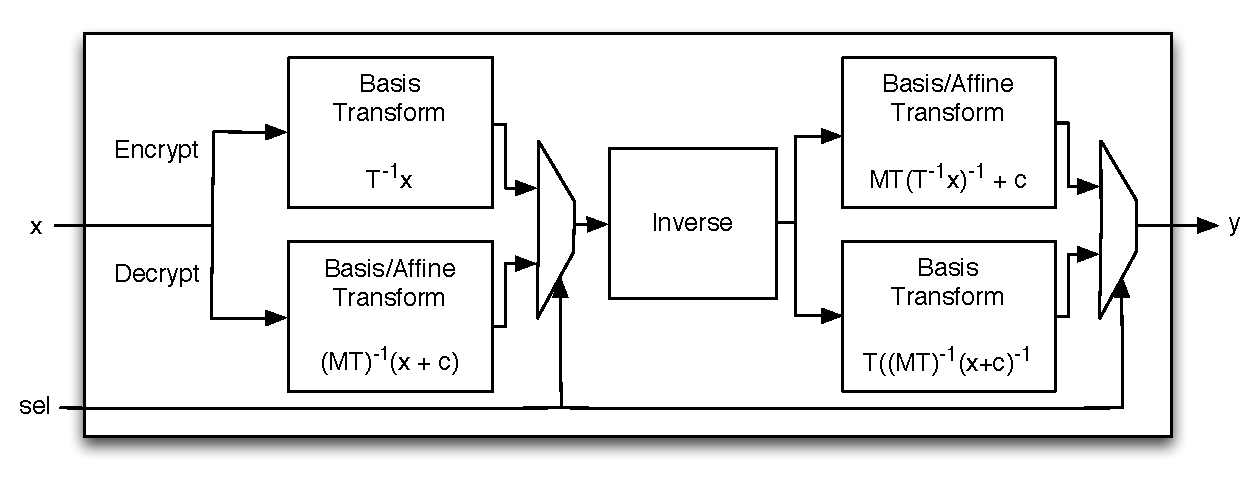
\includegraphics[scale=0.35]{merged_sbox.pdf}
\end{center}
}
\end{frame}

% \begin{frame}
% 	\frametitle{Itoh-Tsujii Inversion (continued)}
% 	\begin{align*}
% 		\alpha^{-1} = (\alpha^r)^{-1}\alpha^{r-1}, \alpha \in GF(q^k), q = 2^n
% 	\end{align*}

% 	\medskip
% 	\pause
% 	Let $NM_1$, $NS_1$, $NM_2$, and $NS_2$ be the number of multiplications and shifts (exponentiations) in $GF(q^k)$ and $GF(q)$, respectively.

% 	\medskip
% 	\pause
% 	This algorithm requires:
% 	\begin{itemize}
% 		\item $NM_1 = \lfloor \log_2(m - 1)\rfloor + HW(m - 1)$,
% 		\item $NS_1 = m - 1$,
% 		\item $NM_2 = \lfloor \log_2(n - 1)\rfloor + HW(n - 1) - 1$, and 
% 		\item $NS_2 = n - 1$,
% 	\end{itemize}
% \end{frame}

% \begin{frame}
% 	\frametitle{Possible Isomorphisms for $GF(2^{16})$}
% $GF(2^{16})$ is isomorphic to $GF((2^n)^m)$ for the following values of $m$ and $n$
% \begin{table}[h]
% \begin{center}
% \label{tab:itaOperations}
% \begin{tabular}{|c|c|c||c|c|c|} \hline
% 	$m$ & $NM_1$ & $NS_1$ & $n$ & $NM_2$ & $NS_2$ \\ \hline
% 	2 & 0 & 1 & 8 & 5 & 7 \\ 
% 	4 & 2 & 3 & 4 & 3 & 3 \\
% 	8 & 4 & 7 & 2 & 1 & 1 \\ \hline 
% \end{tabular}
% \end{center}
% \end{table}

% \pause

% To minimize arithmetic in $GF((2^n)^m)$, we choose $n = 8$ and $m = 2$.

% \end{frame}

% \begin{frame}
% 	\frametitle{Applying the Itoh-Tsujii Inversion Algorithm}
% \begin{itemize}
% 	\item Assume a normal basis for $GF(2^8)$ so that squaring is ``free''
% 	\pause
% 	\item The best known circuit for polynomial multiplication in $GF(2^8)$ requires $69$ XOR and $48$ AND gates
% 	% assume normal basis is more expensive (not taking into account Optimal normal bases)
% 	\pause
% 	\item Squaring in $GF((2^n)^m)$ requires three addition, two squaring, and one scaling operation in the subfield
% 	\pause
% \end{itemize}

% \medskip
% \pause
% The total number of XOR gates required is at least
% \begin{align*}
% 69 \times (5 + 2 + 1) = 552,
% \end{align*}
% which is already more than direct computation in the tower field $GF((((2^2)^2)^2)^2)$.
% \end{frame}

% \begin{frame}[fragile]
% 	\frametitle{Counting Gates for $GF(((2^2)^2)^2)$ Inversion}
% 	Assume a basis $[1, V]$, $[W, W^4]$, and $[X, X^{16}]$ for $GF(((2^2)^2)^2)$.
% 	\begin{itemize}
% 		\item Inversion: $2 \times 2 + 3 \times 4 + 1 = 17$ gates
% 		\item Multiplication: $4 \times 2 + 3 \times 4 + 1 = 21$ gates
% 		\item Square-scale: between $3-5$ gates, depending on the coefficient $\Pi$
% 	\end{itemize}

% \begin{minted}[fontsize=\scriptsize,frame=single]{c}
% > F2 := GF(2);
% > Poly2<V> := PolynomialRing(F2);
% > P := V^2 + V + 1;
% > F4<v> := ext<F2 | P>;
% > Poly4<W> := PolynomialRing(F4);
% > Q := W^2 + W + v;
% > F16<w> := ext<F4 | Q>;
% > Poly16<X> := PolynomialRing(F16);
% > R := X^2 + X + (v + 1)*w + v;
% > F256<x> := ext<F16 | R>;
% > newSigma := changeSigmaRoot(1, v, F4, v);                      
% > newPi := changePiRoot(1, v, w, w^4, F4, F16, (v + 1)*w + v);   
% > gatesInv8(P, Q, R, newSigma, newPi, 1, v, w, w^4, x, x^16);
% 76
% \end{minted}

% \end{frame}

\section{Combinational Logic Minimization}
\begin{frame}
	\frametitle{Changing Gears...}
	\begin{itemize}
		\item To compute the multiplicative inverse of an element in $GF(2^{16})$ using the isomorphic field $GF((((2^2)^2)^2)^2)$.
		\begin{enumerate}
			\item Change from polynomial basis in $GF(2^{16})$ to mixed basis in $GF((((2^2)^2)^2)^2)$
			\item Compute the inverse
			\item Change from mixed basis in $GF((((2^2)^2)^2)^2)$ to polynomial basis in $GF(2^{16})$
		\end{enumerate}
		\pause
		\item There are at least two more opportunities for area improvement
		\begin{enumerate}
			\item Reduce the logic required to change bases (and perform the affine transformation) - these are both linear operations
			\item Reduce the logic required to compute the multiplicative inverse - this is a nonlinear operation
		\end{enumerate}
	\end{itemize}
\end{frame}

% \subsection{Linear Circuit Optimization}
\begin{frame}
	\frametitle{Linear Circuits as Straight Line Programs}
	\begin{itemize}
		\item Consider the following system of linear equations over $GF(2)$:
\begin{align*}
y_1 & = \alpha_{1,1}x_1 + \alpha_{1,2}x_2 + \dots + \alpha_{1,n} \\
y_2 & = \alpha_{2,1}x_1 + \alpha_{2,2}x_2 + \dots + \alpha_{2,n} \\
\dots \\
y_m & = \alpha_{m,1}x_1 + \alpha_{m,2}x_2 + \dots + \alpha_{m,n},
\end{align*}
		\item An SLP is a series of lines of the form $u := v + w$ where $v$ and $w$ are \emph{input variables} $x$ and some $u$ are \emph{output variables} $y$.
		\item Minimizing linear circuits (i.e. circuits with only XOR gates) is equivalent to finding the shortest equivalent \emph{straight line program} (SLP)
	\end{itemize}
\end{frame}


\begin{frame}
	\frametitle{Optimal Straight Line Programs}
	\begin{itemize}
		\item An SLP is \emph{cancellation-free} (i.e. completely factored) if for every line $u := v + w$, $v$ and $w$ do not share any common variables
		\pause 
		\item Optimal cancellation-free SLPs do not always yield optimal SLPs!
{\scriptsize

\begin{columns}[t]
\begin{column}[t]{0.305\linewidth}

\begin{align*}
y_0 & := x_1 + x_2 \\
y_1 & := x_1 + x_2 + x_3 \\
y_2 & := x_1 + x_2 + x_3 + x_4 \\
y_3 & := x_2 + x_3 + x_4 
\end{align*}

\begin{center}
\emph{Original system}
\end{center}

\end{column}

\begin{column}[t]{0.305\linewidth}

\begin{align*}
u_1 & := x_1 + x_2 \: (y_0)\\
u_2 & := u_1 + x_3 \: (y_1)\\
u_3 & := u_2 + x_4 \: (y_2)\\
v_1 & := x_2 + x_3 \\
u_4 & := v_1 + x_4 \: (y_3)
\end{align*}

\begin{center}
\emph{Factored SLP}
\end{center}

\end{column}

\begin{column}[t]{0.305\linewidth}

\begin{align*}
u_1 & := x_1 + x_2 \: (y_0)\\
u_2 & := u_1 + x_3 \: (y_1)\\
u_3 & := u_2 + x_4 \: (y_2)\\
u_4 & := u_3 + x_1 \: (y_3)
\end{align*}

\begin{center}
\emph{Unfactored SLP}
\end{center}

\end{column}

\end{columns}
}
	\end{itemize}

\pause
\begin{center}
\emph{Finding an optimal length SLP is an NP-hard problem}
\end{center}
\end{frame}

\begin{frame}
	\frametitle{Heuristic-Based Optimizations}
	To date, the most effective heuristic-based techniques are:
	\begin{itemize}
		\item Christof Paar's greedy factorization technique \pause \cmark
		\item David Canright's exhaustive factorization \pause \cmark
		\item Daniel Bernstein's Bos-Coster approach \pause \xmark (generated longer SLPs)
		\item Rene Peralta and Joan Boyar's predicate distance-based heuristic \pause \cmark
		\item \emph{Exact} optimizations with SAT-based proofs \pause \xmark (not in scope)
	\end{itemize}
\end{frame}

%%% TODO: describe factorization and boyar-peralta technique

\begin{frame}
	\frametitle{Performance Comparison}
\begin{table}[h]
\begin{center}
	\begin{tabular}{| c | c | c |} \hline
		\emph{Matrix Size} & \emph{Algorithm} & \emph{Average XOR Count} \\ \hline
		$16 \times 16$ & Paar Greedy Factorization & 58.14 \\
		$16 \times 16$ & Boyar-Peralta Optimization \#1 & 50.09 \\
		$16 \times 16$ & Boyar-Peralta Optimization \#2 & 50.11 \\
		$16 \times 16$ & Boyar-Peralta Optimization \#3 & 50.09 \\
		$16 \times 16$ & Boyar-Peralta Optimization \#4 & 53.1 \\
		$16 \times 16$ & Bernstein Optimization & 85.0 \\ \hline
		$32 \times 16$ & Paar Greedy Factorization & 103.89 \\
		$32 \times 16$ & Boyar-Peralta Optimization \#1 & 83.22 \\
		$32 \times 16$ & Boyar-Peralta Optimization \#2 & 83.27 \\
		$32 \times 16$ & Boyar-Peralta Optimization \#3 & 83.22 \\
		$32 \times 16$ & Boyar-Peralta Optimization \#4 & 88.15 \\
		$32 \times 16$ & Bernstein Optimization & 146.66 \\ \hline
	\end{tabular}
\end{center}
\end{table}
\end{frame}

\begin{frame}
	\frametitle{Parallel Implementations of Linear Optimization Techniques}
	The most appealing candidates for improvement are the exhaustive factorization and Boyar-Peralta techniques:
	\begin{itemize}
		\item The factorization search tree can grow exponentially with the input matrix dimensions
		\item Computing new predicate distances in Boyar and Peralta's technique is the bottleneck
	\end{itemize}
\end{frame}

\begin{frame}
	\frametitle{Parallel Exhaustive Factorization Performance}
Pattern: recursive fork/join to distribute the search tree traversal among all available cores.
\begin{table}[h]
\begin{center}
	\begin{tabular}{| c | c | c |} \hline
	$m \times n$ & \emph{Sequential Time (msec)} & \emph{Parallel Time (msec)} \\ \hline
	$7 \times 7$ & 16 & 15 \\ 
	$8 \times 8$ & 16 & 17 \\ 
	$9 \times 9$ & 188 & 79 \\ 
	$10 \times 10$ & 4625 & 1703 \\ 
	$12 \times 6$ & 9 & 9 \\
	$14 \times 7$ & 247 & 93 \\ \hline
	\end{tabular}
\end{center}
\end{table}

\begin{center}
	\emph{Note: difficult to collect more data}
\end{center}

\end{frame}

\begin{frame}
	\frametitle{Parallel Boyar-Peralta Performance}
Pattern: result-parallelism to evenly distribute the predicate distance computations among all possible cores.

\begin{figure}
\centering     %%% not \center
\subfigure[$n \times n$ matrices]{\label{fig:a}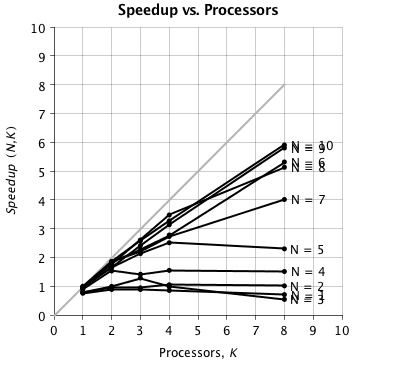
\includegraphics[scale=0.35]{t1u_speed_3.png}}
\subfigure[$2n \times n$ matrices]{\label{fig:b}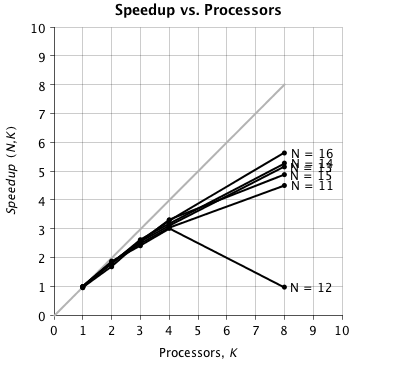
\includegraphics[scale=0.35]{t1m_4.png}}
\end{figure}

% \begin{figure}
% \centering
% \begin{subfigure}{.4\textwidth}
%   \centering
%   \caption{$n \times n$}
% \end{subfigure}%
% \begin{subfigure}{.4\textwidth}
%   \centering
%   \caption{$2n \times n$}
% \end{subfigure}
% \end{figure}

\end{frame}

% \subsection{Nonlinear Circuit Optimization}
% \begin{frame}
% 	\frametitle{Nonlinear Circuit Optimization}
% 	\begin{center}
% 		How can we deterministically transform from one nonlinear function to another equivalent function?
% 	\end{center}

% 	%% TODO: nonlinear circuit picture that shows the hardness of going between two functions
% \end{frame}

% \begin{frame}[fragile]
% 	\frametitle{Ad-Hoc Optimization}
% 	\begin{itemize}
% 		\item Boyar and Peralta also introduced a non-deterministic procedure for optimizing a set of nonlinear equations over $GF(2)$ with the goal of reducing the total required AND gates
% 		\item Start with a set of known signals $S = \{x_1,\dots,x_n\}$ and set of target signals $T = \{f_1,\dots,f_m\}$
% 		\item Pick two random signals $u$ and $v$ from $S$ and do the following:
% 		\begin{itemize}
% 			\item Compute $w = u \oplus v$ ($u \land v$)
% 			\item Check to see if $w$ equals any $f_i \in T$
% 			\item Add $w$ to S
% 			\item Repeat until a maximum depth has been reached, the maximum number of AND (or XOR) gates has been exceeded, or all target functions $T$ have been computed
% 		\end{itemize}
% 		\item If it fails - start over.
% 		\item This is a \emph{randomized} process, so it is not guaranteed to find an answer quickly (if at all!)
% 		\item It's effectiveness is based on the constraints (depth and limit to number of gates)
% 	\end{itemize}
% \end{frame}

% \begin{frame}
% 	\frametitle{Application to Inversion in $GF(2^4)$}
% 	We compared the outcome of this technique (our implementation) against the Synopsys design tool.

% 	\medskip

% 	Interesting note: There are only 8 unique variations from 18 total circuits

% \begin{table}[h]
% \begin{center}
% \tiny
% 	\begin{tabular}{| c | c | c | c | c | c | } \hline  
% 	\emph{Case} & \emph{Field} & $q(w)$ & \emph{Bases} & \emph{SOP (GEs)} & \emph{Ad-Hoc Optimization (GEs)} \\ \hline
% 	1 & $GF((2^2)^2)$ & $w^2 + w + v$ & $[1, V]$ and $[1, W]$         & 26.00 & 51.5      \\
% 	2 & $GF((2^2)^2)$ & $w^2 + w + v$ & $[1, V^2]$ and $[1, W]$       & 27.25 & 49.75     \\
% 	3 & $GF((2^2)^2)$ & $w^2 + w + v$ & $[V, V^2]$ and $[1, W]$       & 31.50 & 44.0      \\
% 	4 & $GF((2^2)^2)$ & $w^2 + w + v$ & $[1, V]$ and $[1, W^4]$       & 26.00 & 51.5      \\
% 	5 & $GF((2^2)^2)$ & $w^2 + w + v$ & $[1, V^2]$ and $[1, W^4]$     & 27.25 & 49.75     \\
% 	6 & $GF((2^2)^2)$ & $w^2 + w + v$ & $[V, V^2]$ and $[1, W^4]$     & 31.50 & 44.0      \\
% 	7 & $GF((2^2)^2)$ & $w^2 + w + v$ & $[1, V]$ and $[W, W^4]$       & 22.75 & 36.75     \\
% 	8 & $GF((2^2)^2)$ & $w^2 + w + v$ & $[1, V^2]$ and $[W, W^4]$     & 20.50 & 22.25     \\
% 	9 & $GF((2^2)^2)$ & $w^2 + w + v$ & $[V, V^2]$ and $[W, W^4]$     & 27.75 & 37.5      \\
% 	10 & $GF((2^2)^2)$ & $w^2 + w + v^2$ & $[1, V]$ and $[1, W]$       & 27.25 & 49.75     \\
% 	11 & $GF((2^2)^2)$ & $w^2 + w + v^2$ & $[1, V^2]$ and $[1, W]$     & 26.00 & 51.5      \\
% 	12 & $GF((2^2)^2)$ & $w^2 + w + v^2$ & $[V, V^2]$ and $[1, W]$     & 29.00 & 41.75     \\
% 	13 & $GF((2^2)^2)$ & $w^2 + w + v^2$ & $[1, V]$ and $[1, W^4]$     & 27.25 & 49.75     \\
% 	14 & $GF((2^2)^2)$ & $w^2 + w + v^2$ & $[1, V^2]$ and $[1, W^4]$   & 26.00 & 51.5      \\
% 	15 & $GF((2^2)^2)$ & $w^2 + w + v^2$ & $[V, V^2]$ and $[1, W^4]$   & 29.00 & 41.75     \\
% 	16 & $GF((2^2)^2)$ & $w^2 + w + v^2$ & $[1, V]$ and $[W, W^4]$     & 20.50 & 22.25     \\
% 	17 & $GF((2^2)^2)$ & $w^2 + w + v^2$ & $[1, V^2]$ and $[W, W^4]$   & 22.75 & 36.75     \\
% 	18 & $GF((2^2)^2)$ & $w^2 + w + v^2$ & $[V, V^2]$ and $[W, W^4]$   & 29.25 & 34.75     \\ \hline
% 	19 & $GF(2^4)$ & $w^4 + w + 1$ & $[1, W, W^2, W^3]$                & 36.50 & NA  \\
% 	20 & $GF(2^4)$ & $w^4 + w^3 + 1$  & $[1, W, W^2, W^3]$             & 22.00 & NA  \\
% 	21 & $GF(2^4)$ & $w^4 + w^3 + w^2 + w + 1$  & $[1, W, W^2, W^3]$   & 26.00 & NA  \\ \hline
% 	\end{tabular}
% \end{center}
% \end{table}
% \end{frame}

% \begin{frame}
% 	\frametitle{Optimization Implications}
% 	Boyar and Peralta's technique was designed to reduce the total number of AND gates (over XOR gates!)

% 	\medskip
% 	\pause

% 	From a transistor perspective, this is the wrong goal!
% 	\begin{itemize}
% 		\item NAND: 4 transistors
% 		\item AND: 6 transistors
% 		\item XOR: 8 transistors
% 	\end{itemize}

% 	\medskip
% 	\pause

% 	\textbf{Future work}: Only use NAND/NOT rounds when finding equivalent nonlinear functions and compare against Synopsys
% \end{frame}

% %%%% COMBINATIONAL LOGIC MINIMIZATION TECHNIQUES
% %    linear: SLP problem, paar factorization, counter example, peralta technique, parallel implementation results
% %    nonlinear: ad-hoc technique, signal graph, application to GF(2^4) inverse

%%% PICKING S-box constructions
% merged circuit with optimized basis change matrices

\section{Main Results}
\begin{frame}
	\frametitle{Putting Everything Together}
	\begin{center}
		Before applying all of these techniques together, let's revisit the AES S-box
	\end{center}
\end{frame}

\begin{frame}
	\frametitle{A Brief History of the AES S-Box}
	\begin{itemize}
		\item (2001) Rudra et al. use the composite field $GF((2^4)^2)$ to reduce the area of the AES S-Box at CHES 2001.
		\pause
		\item (2001) Satoh et al. build upon this result by using the composite field $GF(((2^2)^2)^2)$ with a tower of polynomial bases.
		\pause
		\item(2005) Mentens et al. show that the previous work can be improved with a different selection of irreducible polynomial $r(x)$.
		\pause
		\item (2005) Canright provides an exhaustive search of all $432$ basis representations of $GF(((2^2)^2)^2)$ with low-level arithmetic optimizations.
		\pause
		\item (2008) Nikova et al. use the composite field $GF((2^4)^2)$ with a tower of normal bases to show that the selection of an optimal normal basis in $GF(2^4)$ can yield lower GEs than Canright's construction (in some cases).
		\pause
		\item (2011-2013) Boyar and Peralta used their novel combinational logic minimization techniques for linear and nonlinear circuits to improve Canright's construction to 32 AND and 83 XOR/XNOR gates.
		\item ... and our work
	\end{itemize}
\end{frame}

\begin{frame}
	\frametitle{A New Look at the AES S-Box}
	\begin{itemize}
		% \item We found a set of basis change matrices that were smaller than Canright's by a single XOR gate using Boyar and Peralta's minimization technique (they do however have the same nonzero element count as Canright's matrices when unoptimized):
		\item A set of basis change matrices different from the ones used by Canright
		\item Parameters:
		\begin{itemize}
			\item $GF(2^8)$ polynomial: $p(v) = v^8 + v^4 + v^3 + v + 1$ (AES field polynomial)
			\item Tower of normal bases with the same coefficients $\Sigma$ and $\Pi$ as Canright: $\Sigma = v^2$ and $\Pi = vw$
		\end{itemize}
	\end{itemize}
\begin{align*}
\mathbf{T} = 
\begin{pmatrix}
0 & 0 & 0 & 1 & 0 & 0 & 1 & 0 \\
1 & 1 & 1 & 0 & 1 & 0 & 1 & 1 \\
1 & 1 & 1 & 0 & 1 & 1 & 0 & 1 \\
0 & 1 & 0 & 0 & 0 & 0 & 1 & 0 \\
0 & 1 & 1 & 1 & 1 & 1 & 1 & 0 \\
1 & 0 & 1 & 1 & 0 & 0 & 1 & 0 \\
0 & 0 & 1 & 0 & 0 & 0 & 1 & 0 \\
0 & 0 & 0 & 0 & 0 & 1 & 0 & 0 \\
\end{pmatrix}
\;
\mathbf{T}^{-1} = 
\begin{pmatrix}
1 & 1 & 1 & 0 & 0 & 1 & 1 & 1 \\
0 & 1 & 1 & 1 & 0 & 0 & 0 & 1 \\
0 & 1 & 1 & 0 & 0 & 0 & 1 & 1 \\
1 & 1 & 1 & 0 & 0 & 0 & 0 & 1 \\
1 & 0 & 0 & 1 & 1 & 0 & 1 & 1 \\
0 & 0 & 0 & 0 & 0 & 0 & 0 & 1 \\
0 & 1 & 1 & 0 & 0 & 0 & 0 & 1 \\
0 & 1 & 0 & 0 & 1 & 1 & 1 & 1 \\
\end{pmatrix}
\end{align*}

	\begin{center}
		\textbf{Implication}: Canright didn't explore all possible isomorphisms between standard AES representation and mixed basis composite representation - can we still do better for the AES S-box?
	\end{center}

\end{frame}

\begin{frame}
	\frametitle{AES S-Box Alternative}
	If we use the $GF(2^8)$ field polynomial $s(v) = v^8 + v^6 + v^5 + v^4 + v^2 + v + 1$, a possible S-box with low area requirements (103 XOR and 36 AND gates without logic optimizations similar to Canright) is as follows:

\begin{align*}
S(x) =  
\begin{pmatrix}
0 & 0 & 0 & 0 & 1 & 1 & 0 & 1 \\
1 & 1 & 0 & 0 & 1 & 0 & 1 & 1 \\
0 & 0 & 1 & 0 & 0 & 1 & 1 & 1 \\
0 & 1 & 0 & 0 & 1 & 1 & 1 & 1 \\
1 & 1 & 0 & 0 & 0 & 0 & 0 & 0 \\
1 & 0 & 0 & 1 & 1 & 0 & 0 & 0 \\
0 & 0 & 0 & 0 & 1 & 1 & 0 & 0 \\
1 & 0 & 0 & 0 & 1 & 0 & 1 & 0 \\
\end{pmatrix}
\begin{pmatrix}
x_7 \\
x_6 \\
x_5 \\
x_4 \\
x_3 \\ 
x_2 \\
x_1 \\
x_0 \\
\end{pmatrix}^{-1}
+
\begin{pmatrix}
0 \\
0 \\
0 \\
0 \\
1 \\ 
0 \\
0 \\
0 \\
\end{pmatrix}
\end{align*}
\end{frame}

\begin{frame}
	\frametitle{Other Suitable Power Mappings}
	\begin{itemize}
		\item What if we don't want to use the inverse mapping?
		\item There are other power mapping exponents $d$ (and inverses $d^{-1}$) with high nonlinearity ($112$) and low differential uniformity ($4$):
		\begin{itemize}
			\itemsep0em
			\item $d = 127$, $d^{-1} = 253$
			\item $d = 191$, $d^{-1} = 251$
			\item $d = 223$, $d^{-1} = 247$
			\item $d = 239$, $d^{-1} = 239$
			\item $d = 247$, $d^{-1} = 223$
			\item $d = 251$, $d^{-1} = 191$
			\item $d = 253$, $d^{-1} = 127$
			\item $d = 254$, $d^{-1} = 254$
		\end{itemize}
		\item We did not explore implementations of S-boxes based on these power mappings
	\end{itemize}
\end{frame}

\begin{frame}
	\frametitle{16-Bit S-Box Results}
	Our best candidate has the following parameters:
	\begin{itemize}
		\item Field polynomial: $t(v) = v^{16} + v^5 + v^3 + v + 1$
		\item Basis sets: $[1, V]$, $[1, W]$, $[1, X]$, and $[Y^{256}, Y]$
		\item Coefficients: $\Sigma = v$, $\Pi = vw + v$, and $\Lambda = (vw + v)x + w$
	\end{itemize}

	\begin{itemize}
		\item Our (unoptimized) version of this S-box requires $1238$ XOR gates and $144$ AND gates 
		\item This can clearly be improved by applying Boyar and Peralta's optimization techniques
	\end{itemize}
\end{frame}

\begin{frame}
	\frametitle{16-Bit S-Box Definition}
\small
\begin{align*}
S(x) =  
\begin{pmatrix}
0 & 0 & 1 & 0 & 0 & 0 & 0 & 1 & 0 & 0 & 1 & 1 & 1 & 1 & 1 & 0 \\
1 & 1 & 0 & 0 & 0 & 0 & 0 & 1 & 0 & 1 & 1 & 0 & 1 & 0 & 1 & 0 \\
1 & 1 & 0 & 0 & 1 & 0 & 1 & 1 & 0 & 1 & 0 & 1 & 0 & 0 & 1 & 1 \\
1 & 1 & 1 & 0 & 0 & 0 & 1 & 0 & 0 & 1 & 1 & 0 & 0 & 0 & 0 & 0 \\
1 & 1 & 0 & 0 & 0 & 1 & 1 & 0 & 0 & 1 & 1 & 1 & 1 & 0 & 1 & 1 \\
0 & 1 & 0 & 0 & 0 & 0 & 1 & 1 & 0 & 1 & 1 & 1 & 1 & 1 & 0 & 1 \\
0 & 0 & 1 & 0 & 1 & 0 & 1 & 0 & 1 & 1 & 0 & 0 & 1 & 1 & 0 & 0 \\
1 & 0 & 1 & 1 & 1 & 0 & 1 & 1 & 0 & 0 & 0 & 1 & 0 & 1 & 1 & 1 \\
0 & 1 & 0 & 0 & 0 & 0 & 0 & 0 & 1 & 0 & 0 & 1 & 1 & 1 & 0 & 1 \\
1 & 0 & 1 & 1 & 0 & 0 & 0 & 1 & 0 & 0 & 1 & 0 & 1 & 0 & 0 & 0 \\
1 & 0 & 1 & 0 & 0 & 1 & 1 & 1 & 0 & 0 & 1 & 1 & 0 & 1 & 0 & 0 \\
1 & 0 & 1 & 1 & 1 & 0 & 1 & 1 & 1 & 1 & 0 & 1 & 1 & 0 & 0 & 1 \\
1 & 0 & 1 & 0 & 0 & 1 & 0 & 1 & 1 & 0 & 0 & 1 & 0 & 0 & 0 & 1 \\
0 & 1 & 0 & 0 & 0 & 1 & 1 & 1 & 1 & 0 & 0 & 0 & 0 & 0 & 0 & 1 \\
1 & 0 & 0 & 0 & 1 & 1 & 0 & 1 & 0 & 1 & 1 & 1 & 1 & 0 & 0 & 0 \\
1 & 1 & 0 & 1 & 0 & 1 & 1 & 0 & 1 & 0 & 0 & 1 & 1 & 0 & 0 & 0 \\
\end{pmatrix}
\begin{pmatrix}
x_{15} \\
x_{14} \\
x_{13} \\
x_{12} \\
x_{11} \\
x_{10} \\
x_{9} \\
x_{8} \\
x_{7} \\
x_{6} \\
x_{5} \\
x_{4} \\
x_{3} \\
x_{2} \\
x_{1} \\
x_{0} \\
\end{pmatrix}^{-1}
+
\begin{pmatrix}
0 \\
1 \\
0 \\
0 \\
0 \\ 
1 \\
0 \\
1 \\
1 \\
0 \\
1 \\
1 \\
0 \\ 
1 \\
1 \\
1 \\
\end{pmatrix}
% [ 0, 1, 0, 0, 0, 1, 0, 1, 1, 0, 1, 1, 0, 1, 1, 1 ]
\end{align*}
\normalsize
\end{frame}

\begin{frame}
	\frametitle{16-Bit S-Box Basis Change Matrices}
\small
\begin{align*}
\mathbf{T}^{-1} = 
\begin{pmatrix}
1 &0 &1 &0 &0 &0 &0 &1 &1 &0 &0 &0 &0 &0 &1 &0\\
1 &0 &0 &0 &1 &0 &0 &0 &0 &1 &0 &0 &1 &1 &0 &0\\
1 &1 &0 &0 &1 &0 &0 &0 &1 &1 &0 &1 &1 &0 &1 &0\\
0 &1 &1 &1 &1 &0 &1 &1 &1 &0 &1 &1 &1 &0 &0 &0\\
0 &0 &0 &1 &1 &0 &0 &1 &0 &0 &0 &1 &1 &0 &0 &0\\
0 &1 &0 &1 &1 &0 &1 &0 &1 &0 &0 &0 &0 &1 &1 &0\\
1 &0 &1 &1 &0 &0 &1 &1 &0 &0 &0 &1 &1 &1 &0 &0\\
1 &0 &0 &0 &1 &0 &0 &0 &0 &0 &1 &0 &0 &0 &0 &1\\
0 &0 &0 &0 &1 &0 &0 &1 &1 &0 &0 &0 &0 &0 &1 &0\\
1 &0 &1 &0 &0 &0 &1 &1 &0 &1 &0 &1 &1 &0 &1 &0\\
1 &0 &1 &0 &0 &0 &0 &0 &0 &1 &0 &0 &1 &0 &0 &0\\
0 &0 &0 &1 &1 &0 &1 &0 &1 &0 &1 &1 &1 &0 &1 &0\\
0 &0 &0 &0 &1 &1 &1 &1 &0 &1 &1 &0 &0 &0 &0 &0\\
0 &1 &1 &1 &1 &0 &1 &0 &0 &1 &1 &1 &0 &1 &1 &0\\
0 &1 &1 &0 &1 &0 &1 &1 &0 &0 &1 &0 &1 &0 &0 &0\\
1 &1 &0 &1 &0 &0 &0 &0 &0 &0 &1 &1 &1 &0 &1 &1\\
\end{pmatrix}
\end{align*}
\normalsize
\end{frame}

\section{Future Work}
\begin{frame}
	\frametitle{Future Work}
	\begin{enumerate}
		\item AES S-box
		\begin{itemize}
			\item Exhaustively generate all basis change matrices
			\item Use Canright's inversion circuit counts to determine the total cost of the S-box unoptimized
			\item Apply Boyar and Peralta's technique to see if the area and depth can be reduced below the current best-known result
		\end{itemize}
		\pause
		\item Apply combinational logic minimization techniques to other cryptographic problems:
		\begin{itemize}
			\item Low weight and depth binary polynomial multiplication
			\item Efficient 2-party secure computation protocols
			\item NAND/NOT round modifications for CMOS-efficient nonlinear circuits
		\end{itemize}
		\pause
		\item Galois field arithmetic library
		\begin{itemize}
			\item Support flexible polynomial and normal basis arithmetic for arbitrary composite fields and any number of extensions (already started!)
			\item Add symbolic evaluation to programmatically search for and eliminate common subexpressions in all relevant arithmetic expressions
		\end{itemize}
	\end{enumerate}
\end{frame}

\begin{frame}
	\frametitle{Wrapping Up}
	Special thanks to:
	\begin{itemize}
		\item Staszek, Marcin, Alan, and Michael
		\item RIT, GCCIS, and Harris RF
		\item Mats Rynge and the OSG
		\item David Canright, Rene Peralta (NIST), Christof Paar, Nele Mentens
		\item Family and friends
	\end{itemize}
\end{frame}

\begin{frame}
	\frametitle{Questions?}
	\begin{center}
		Fire away!
	\end{center}
\end{frame}

%%% RESULTS
% AES S-boxes
% 16-bit S-box

% Definitions: Boolean functions, finite fields, etc
% strength as measure of resistance to these attacks, and algorithms for doing so
% What about traditional Boolean functions?
% S-box constructions (power mapping, ruled out alternatives by NL check and proof, non-Galois field constructions)
% Definitions: composite fields, bases, etc
% Focus on the inverse power mapping, computation with ITA and straight calculation (discuss ITA complexity)
%    show circuits for inverse calculation
% Combinational logic minimization techniques
%    linear: SLP problem, paar factorization, counter example, peralta technique, parallel implementation results
%    nonlinear: ad-hoc technique, signal graph, application to GF(2^4) inverse
% AES alternative S-boxes, include best option with security measurements
% 16-bit S-boxes, include best option with circuit and whatnot

\end{document}
